\documentclass{article}
\usepackage[utf8]{inputenc}


\font\myfont=cmr12 at 25pt
%\title{\myfont Notes on Permanent Magnet Synchronous Machine (PMSM) Model %Predictive Control (MPC) and Operation Under Open Circuit Fault}
\font\hisfont=cmr12 at 15pt

\author{\hisfont Hakan Saraç}
\date{}


\usepackage{float}
\usepackage{comment}
\usepackage{natbib}
\usepackage{graphicx}
\usepackage{indentfirst}
\usepackage{siunitx}
\usepackage{svg}
\usepackage{hyperref}
\usepackage{amsmath, bm}
\usepackage{graphicx} 
\usepackage{pstool}
\usepackage{listings}
\usepackage{natbib}
\usepackage{graphicx}
\usepackage{epstopdf}
\usepackage{tikz}
\usepackage[utf8]{inputenc}
\usepackage{pgfplots} 
\usepackage{pgfgantt}
\usepackage{pdflscape}
\pgfplotsset{compat=newest} 
\pgfplotsset{plot coordinates/math parser=false}
\lstloadlanguages{Matlab}%
\lstset{ 
	language=Matlab,                		% choose the language of the code
%	basicstyle=10pt,       				% the size of the fonts that are used for the code
	numbers=left,                  			% where to put the line-numbers
	numberstyle=\footnotesize,      		% the size of the fonts that are used for the line-numbers
	stepnumber=1,                   			% the step between two line-numbers. If it's 1 each line will be numbered
	numbersep=5pt,                  		% how far the line-numbers are from the code
%	backgroundcolor=\color{white},  	% choose the background color. You must add \usepackage{color}
	showspaces=false,               		% show spaces adding particular underscores
	showstringspaces=false,         		% underline spaces within strings
	showtabs=false,                 			% show tabs within strings adding particular underscores
%	frame=single,	                			% adds a frame around the code
%	tabsize=2,                				% sets default tabsize to 2 spaces
%	captionpos=b,                   			% sets the caption-position to bottom
	breaklines=true,                			% sets automatic line breaking
	breakatwhitespace=false,        		% sets if automatic breaks should only happen at whitespace
	escapeinside={\%*}{*)}          		% if you want to add a comment within your code
}

\addtolength{\oddsidemargin}{-.875in}
\addtolength{\evensidemargin}{-.875in}
\addtolength{\textwidth}{1.75in}
\addtolength{\topmargin}{-.875in}
\addtolength{\textheight}{1.75in}


\begin{document}
\title{\line(1,0){250}\\\myfont Torque Sharing Report\\\line(1,0){250}}
\maketitle
\newpage
\tableofcontents
\newpage


\section{Introduction}
I have implemented torque sharing using three different approaches. In this document, I have collected the results for evaluation.


\section{Equal Torque Distribution Between Modules}
\begin{figure}[H]
\centering
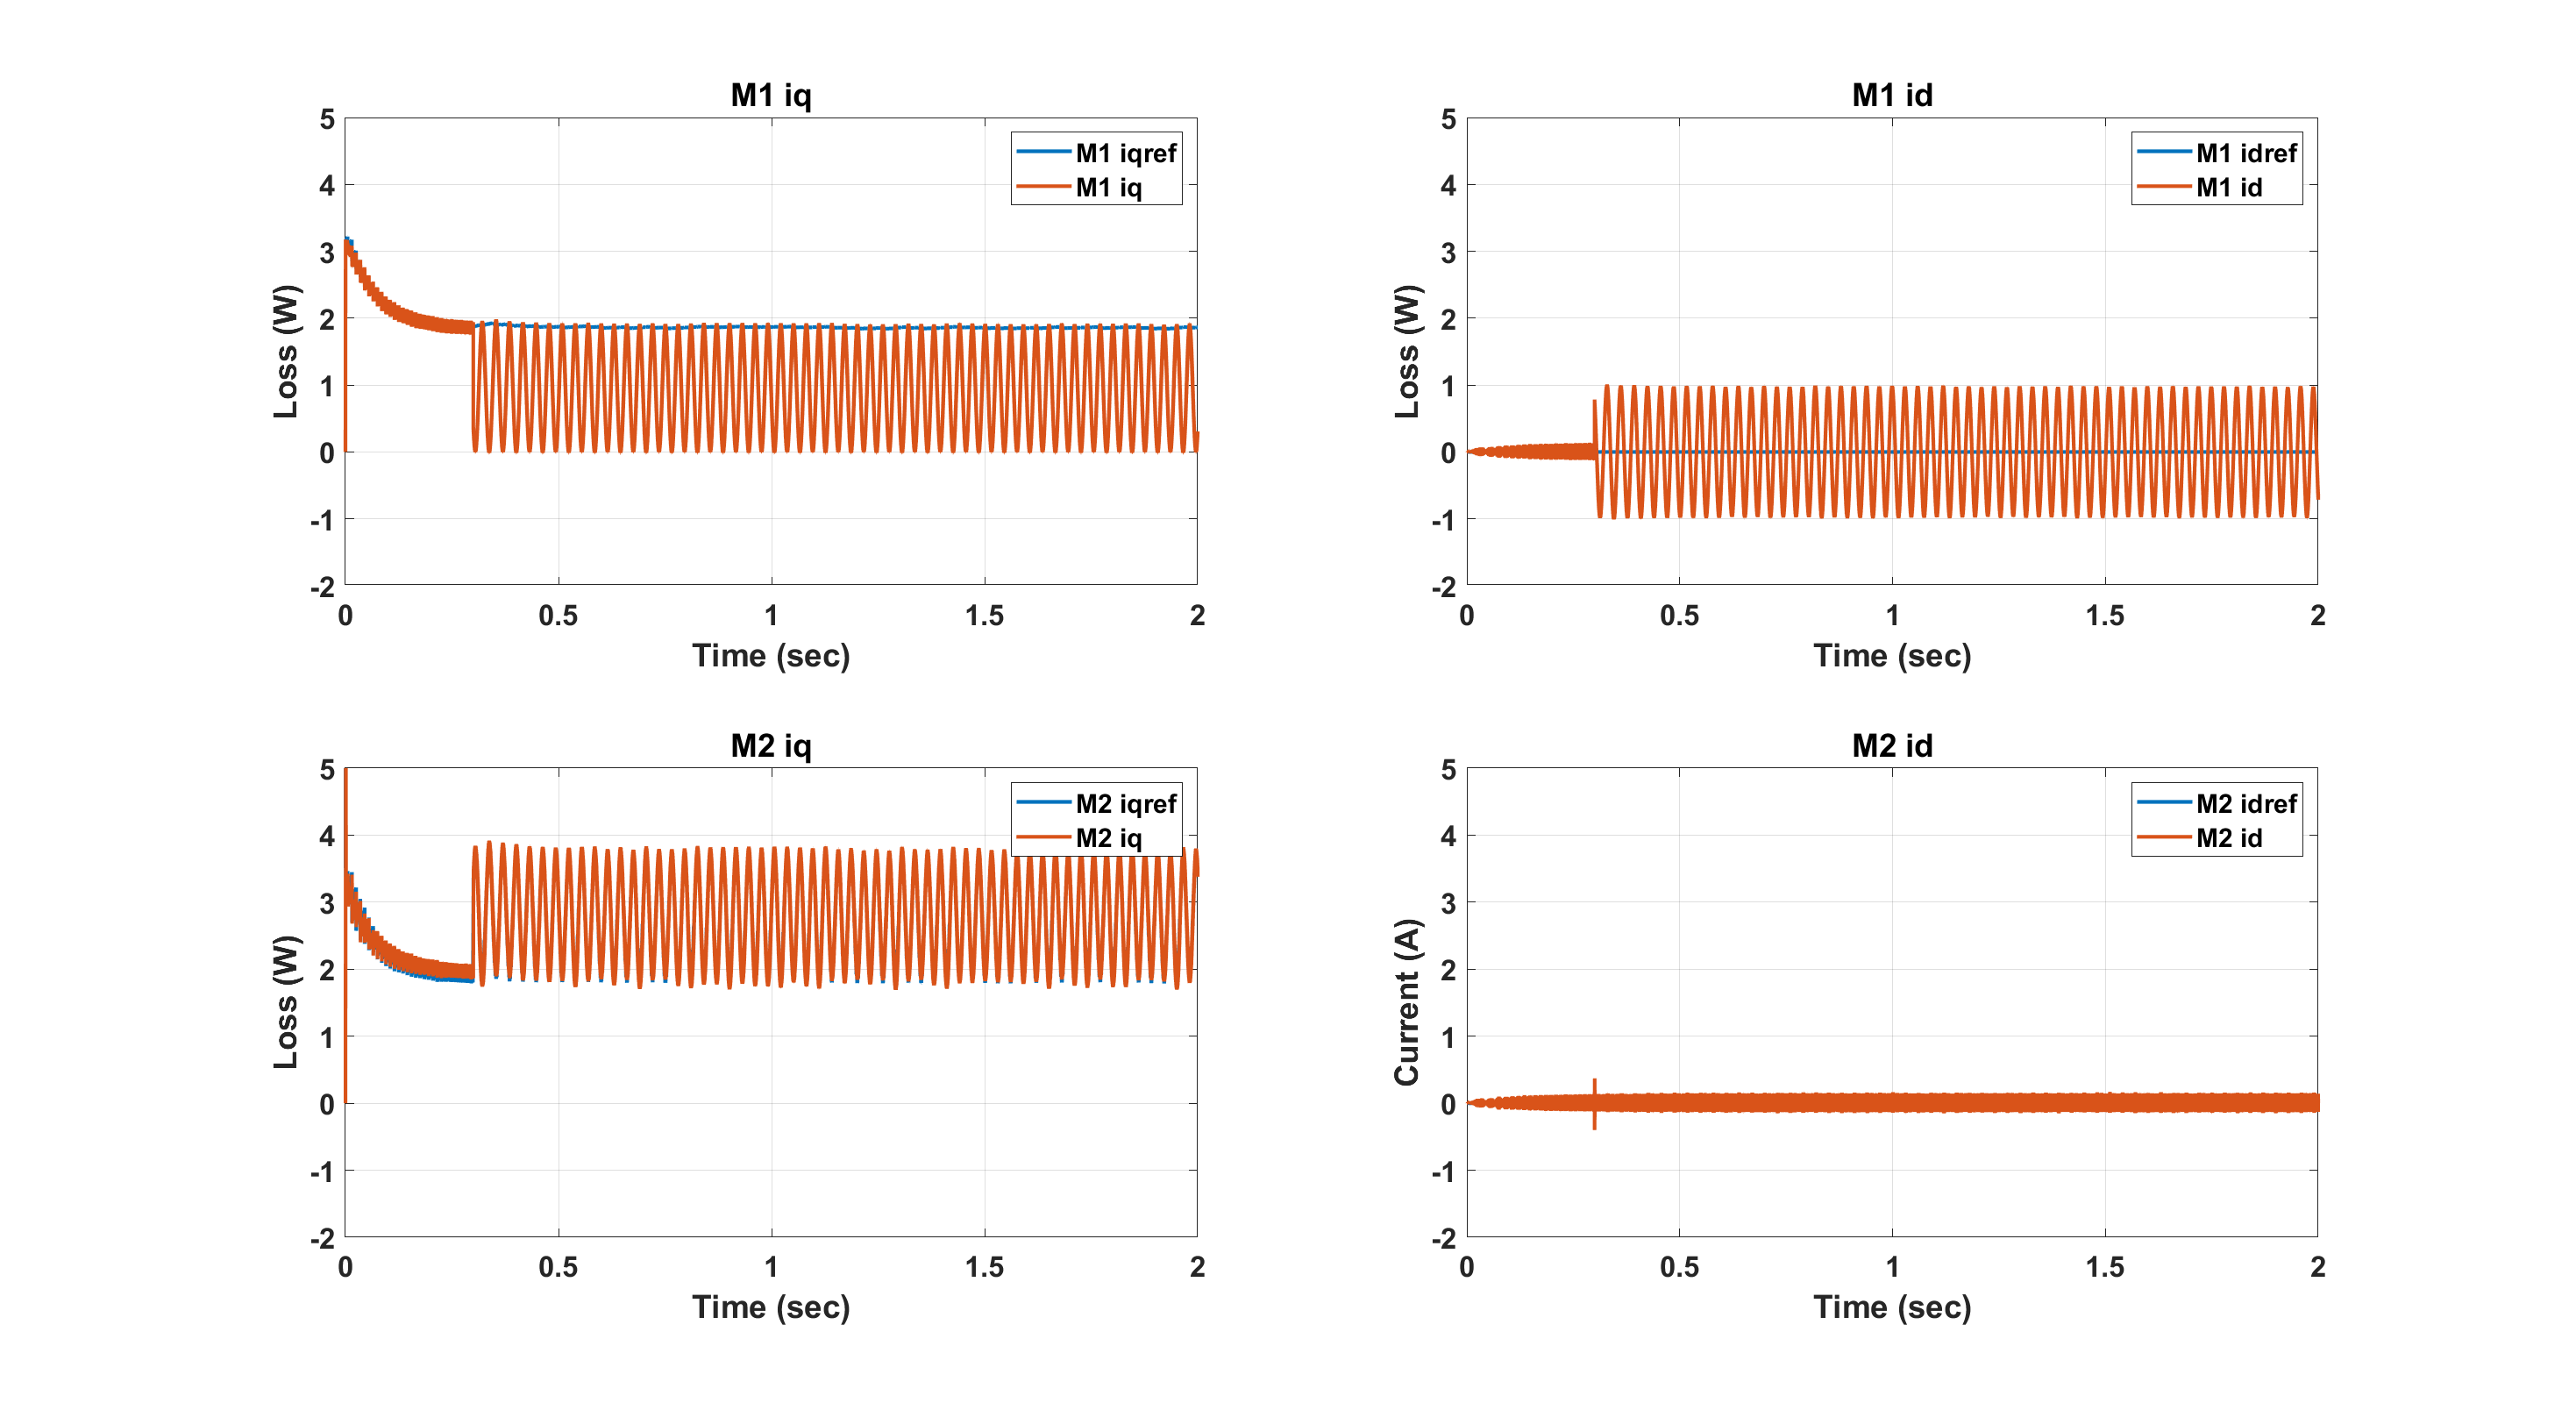
\includegraphics[scale=0.35]{SimulationResults/EqualTorqueShare/idq_refs.eps}
\caption{dq Phase Currents and References for Equal Torque Distribution}
\label{fig:PhaseCurrentsReferencesEqual}
\end{figure}

\begin{figure}[H]
\centering
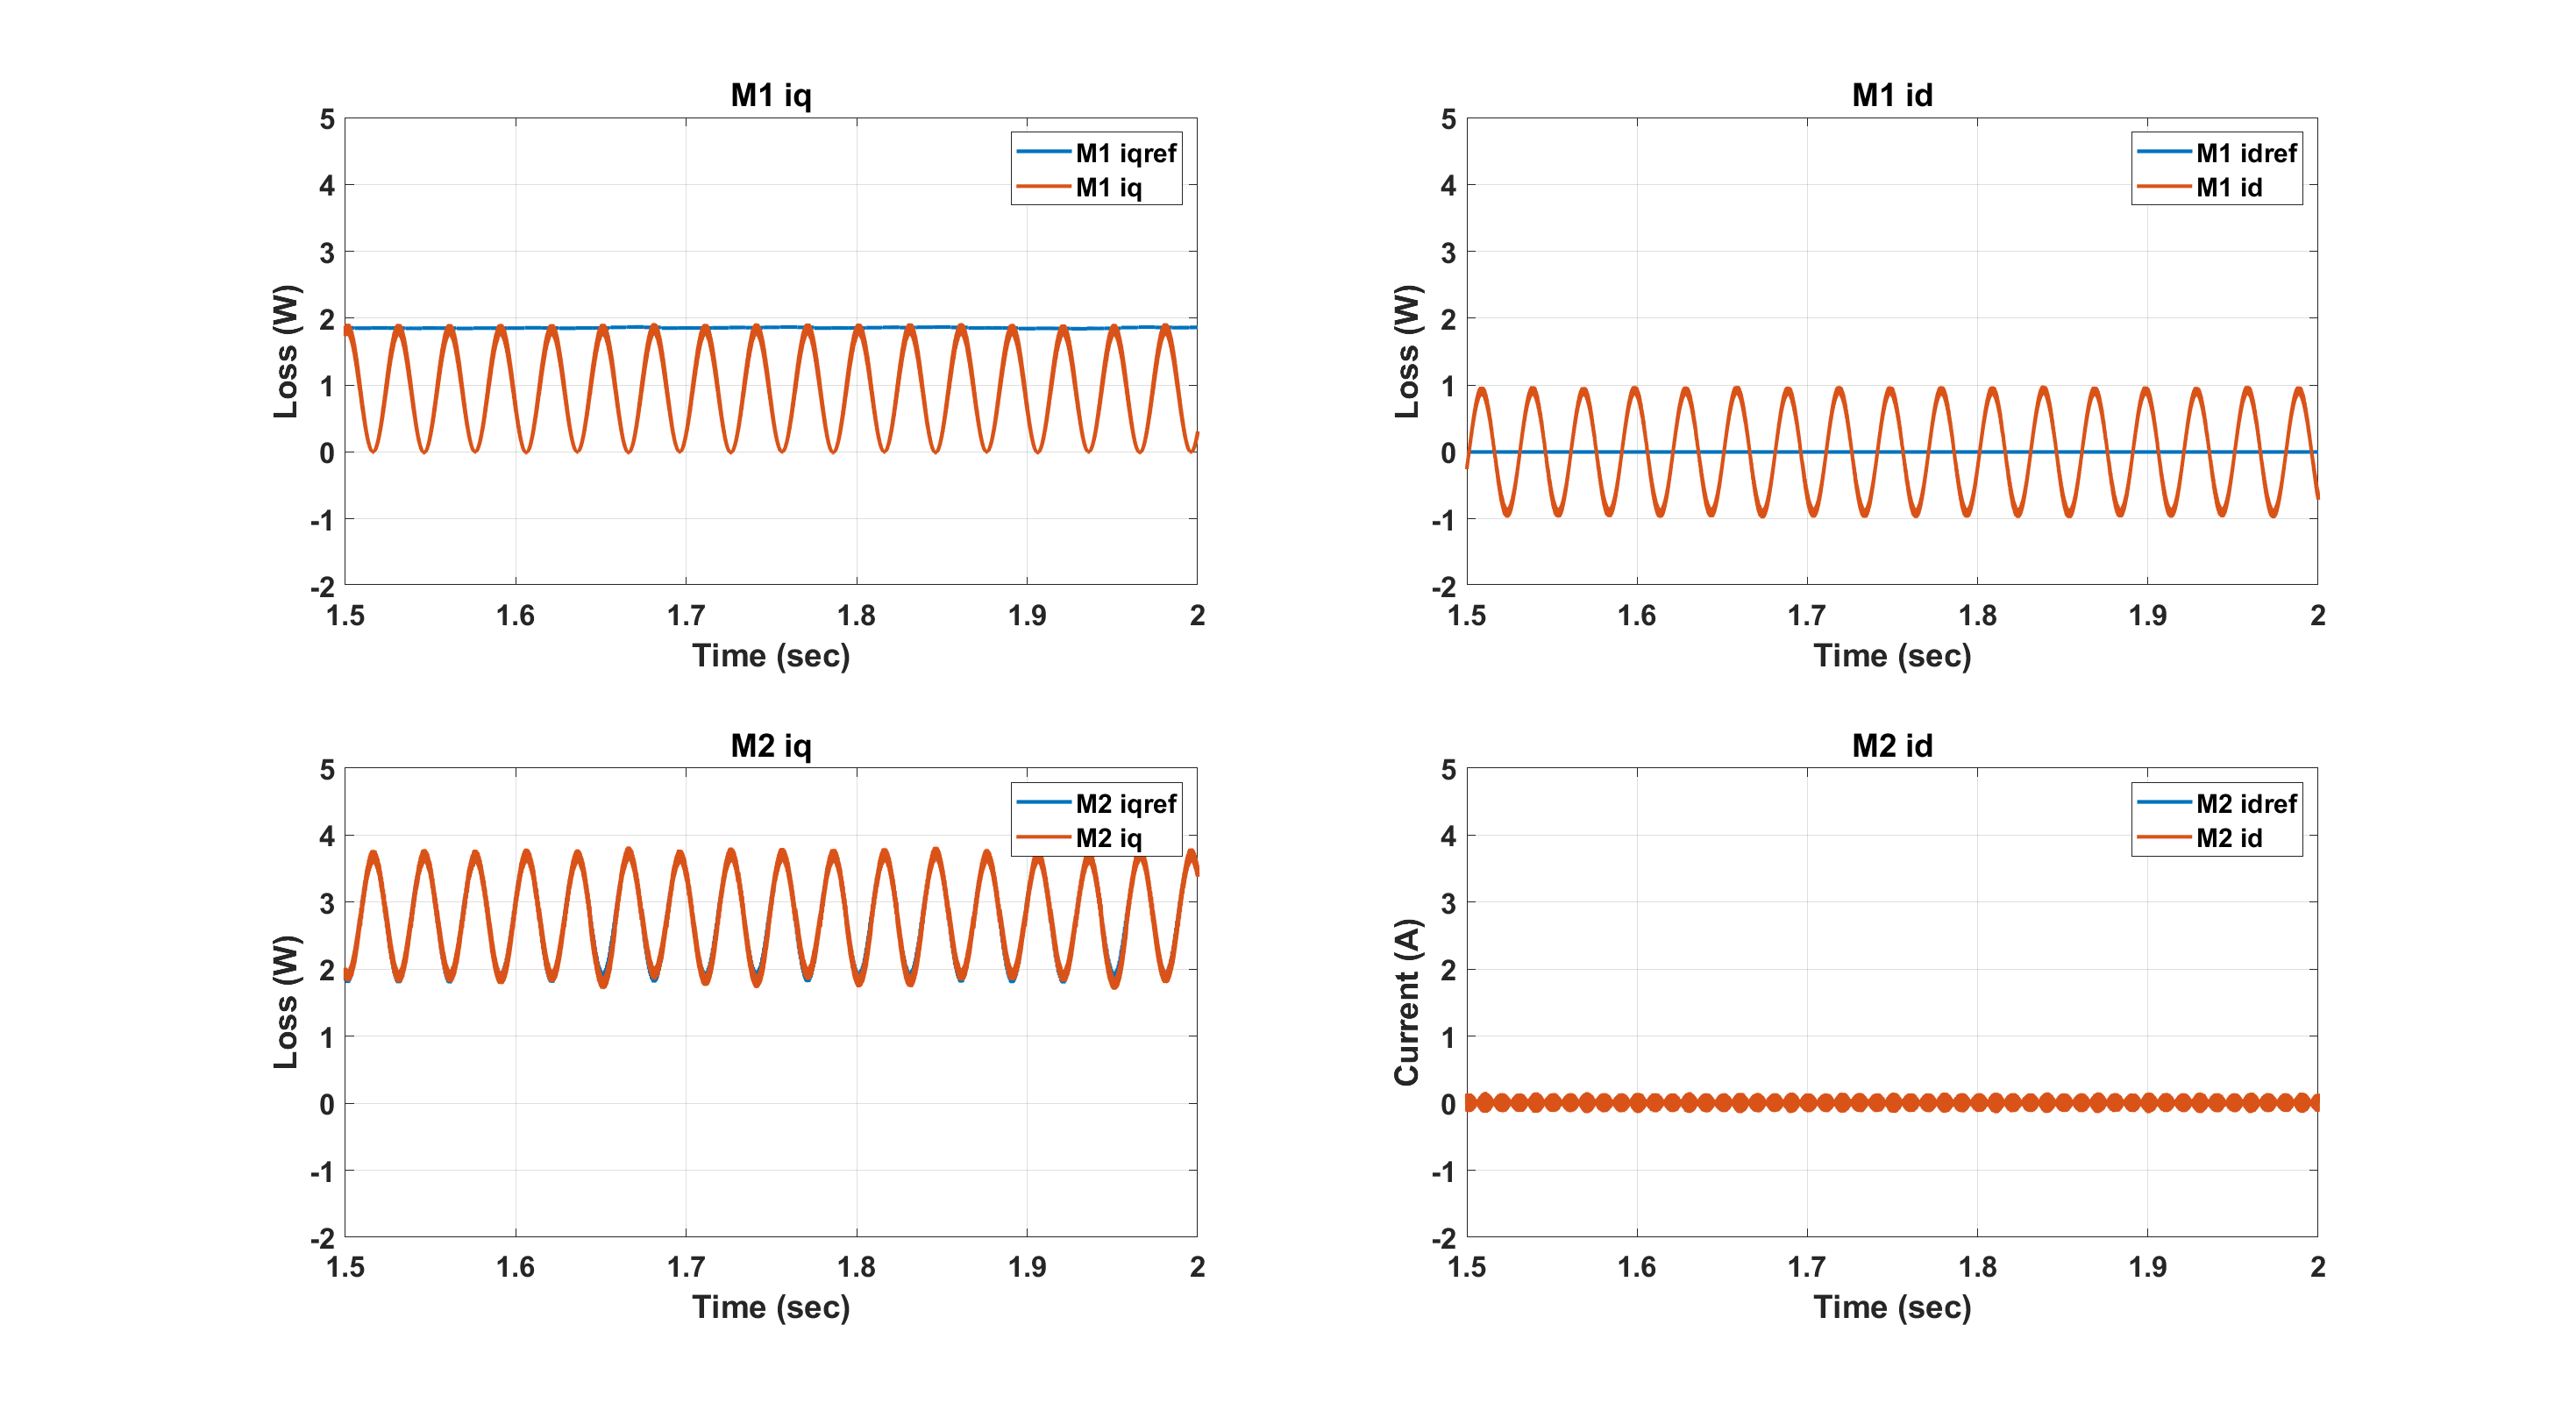
\includegraphics[scale=0.35]{SimulationResults/EqualTorqueShare/idq_refs_closer.eps}
\caption{dq Phase Currents and References for Equal Torque Distribution Closer}
\label{fig:PhaseCurrentsReferencesEqualCloser}
\end{figure}

\begin{figure}[H]
\centering
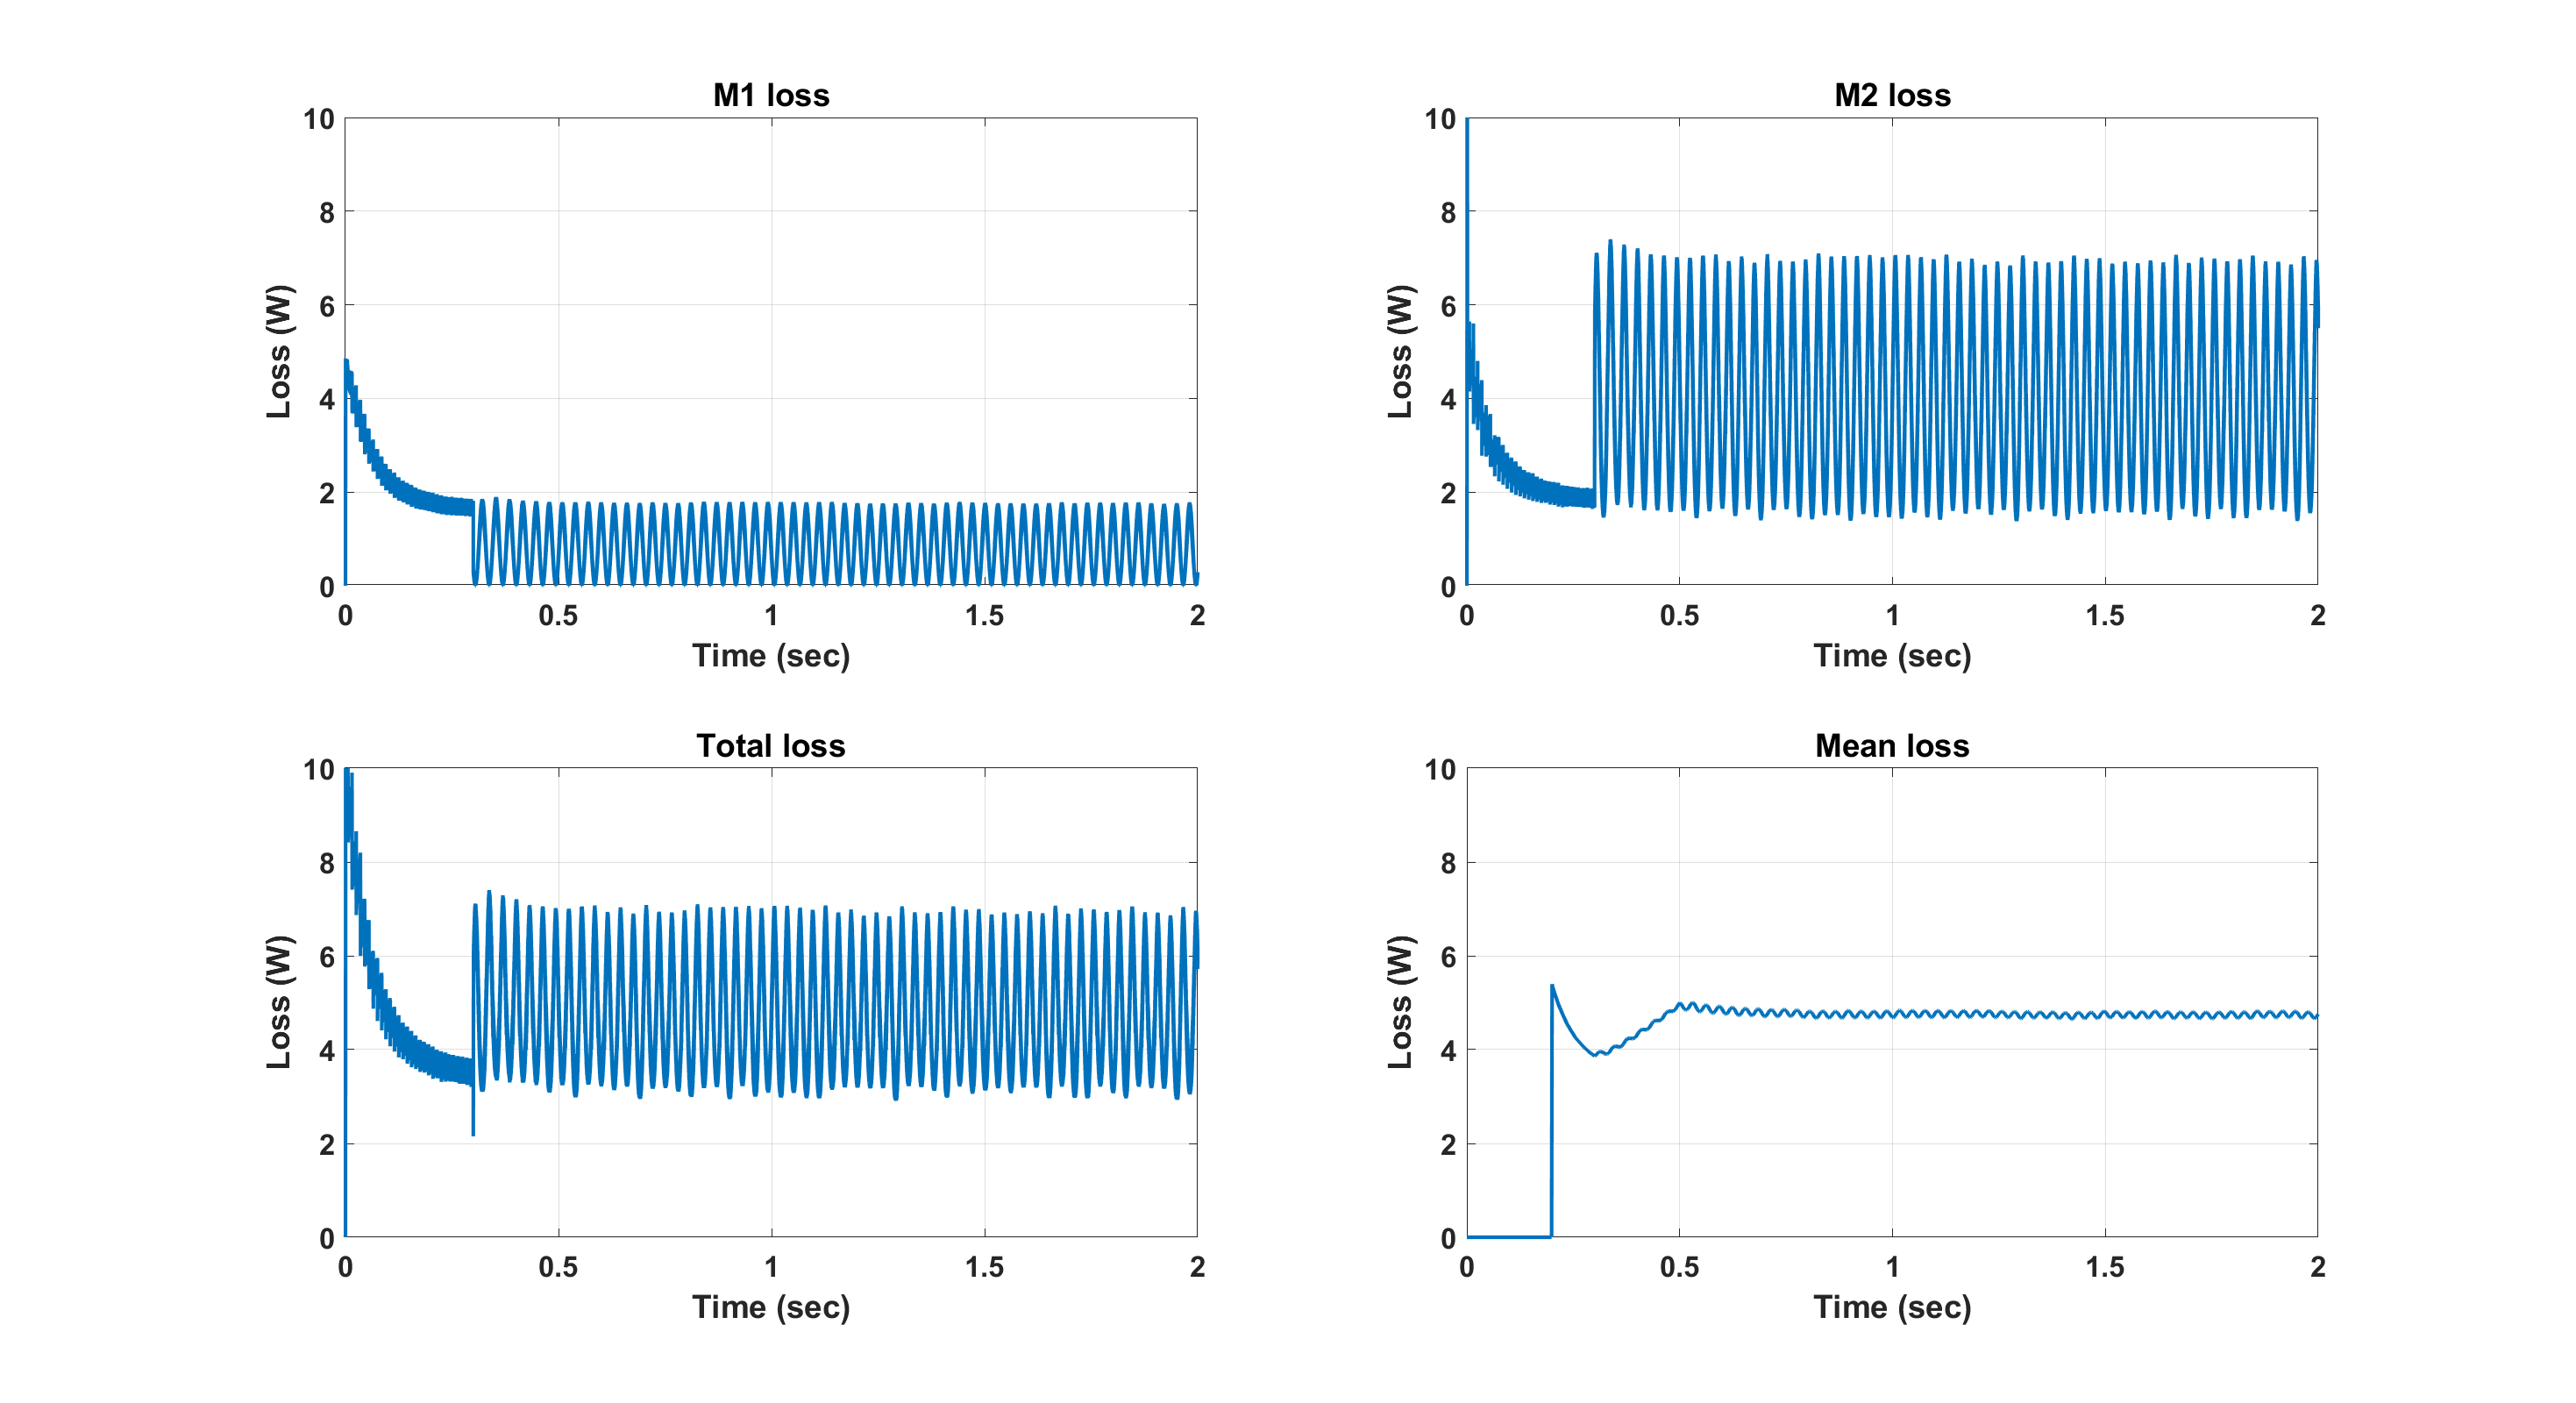
\includegraphics[scale=0.35]{SimulationResults/EqualTorqueShare/Loss.eps}
\caption{Module Losses for Equal Torque Distribution}
\label{fig:LossEqual}
\end{figure}

\begin{figure}[H]
\centering
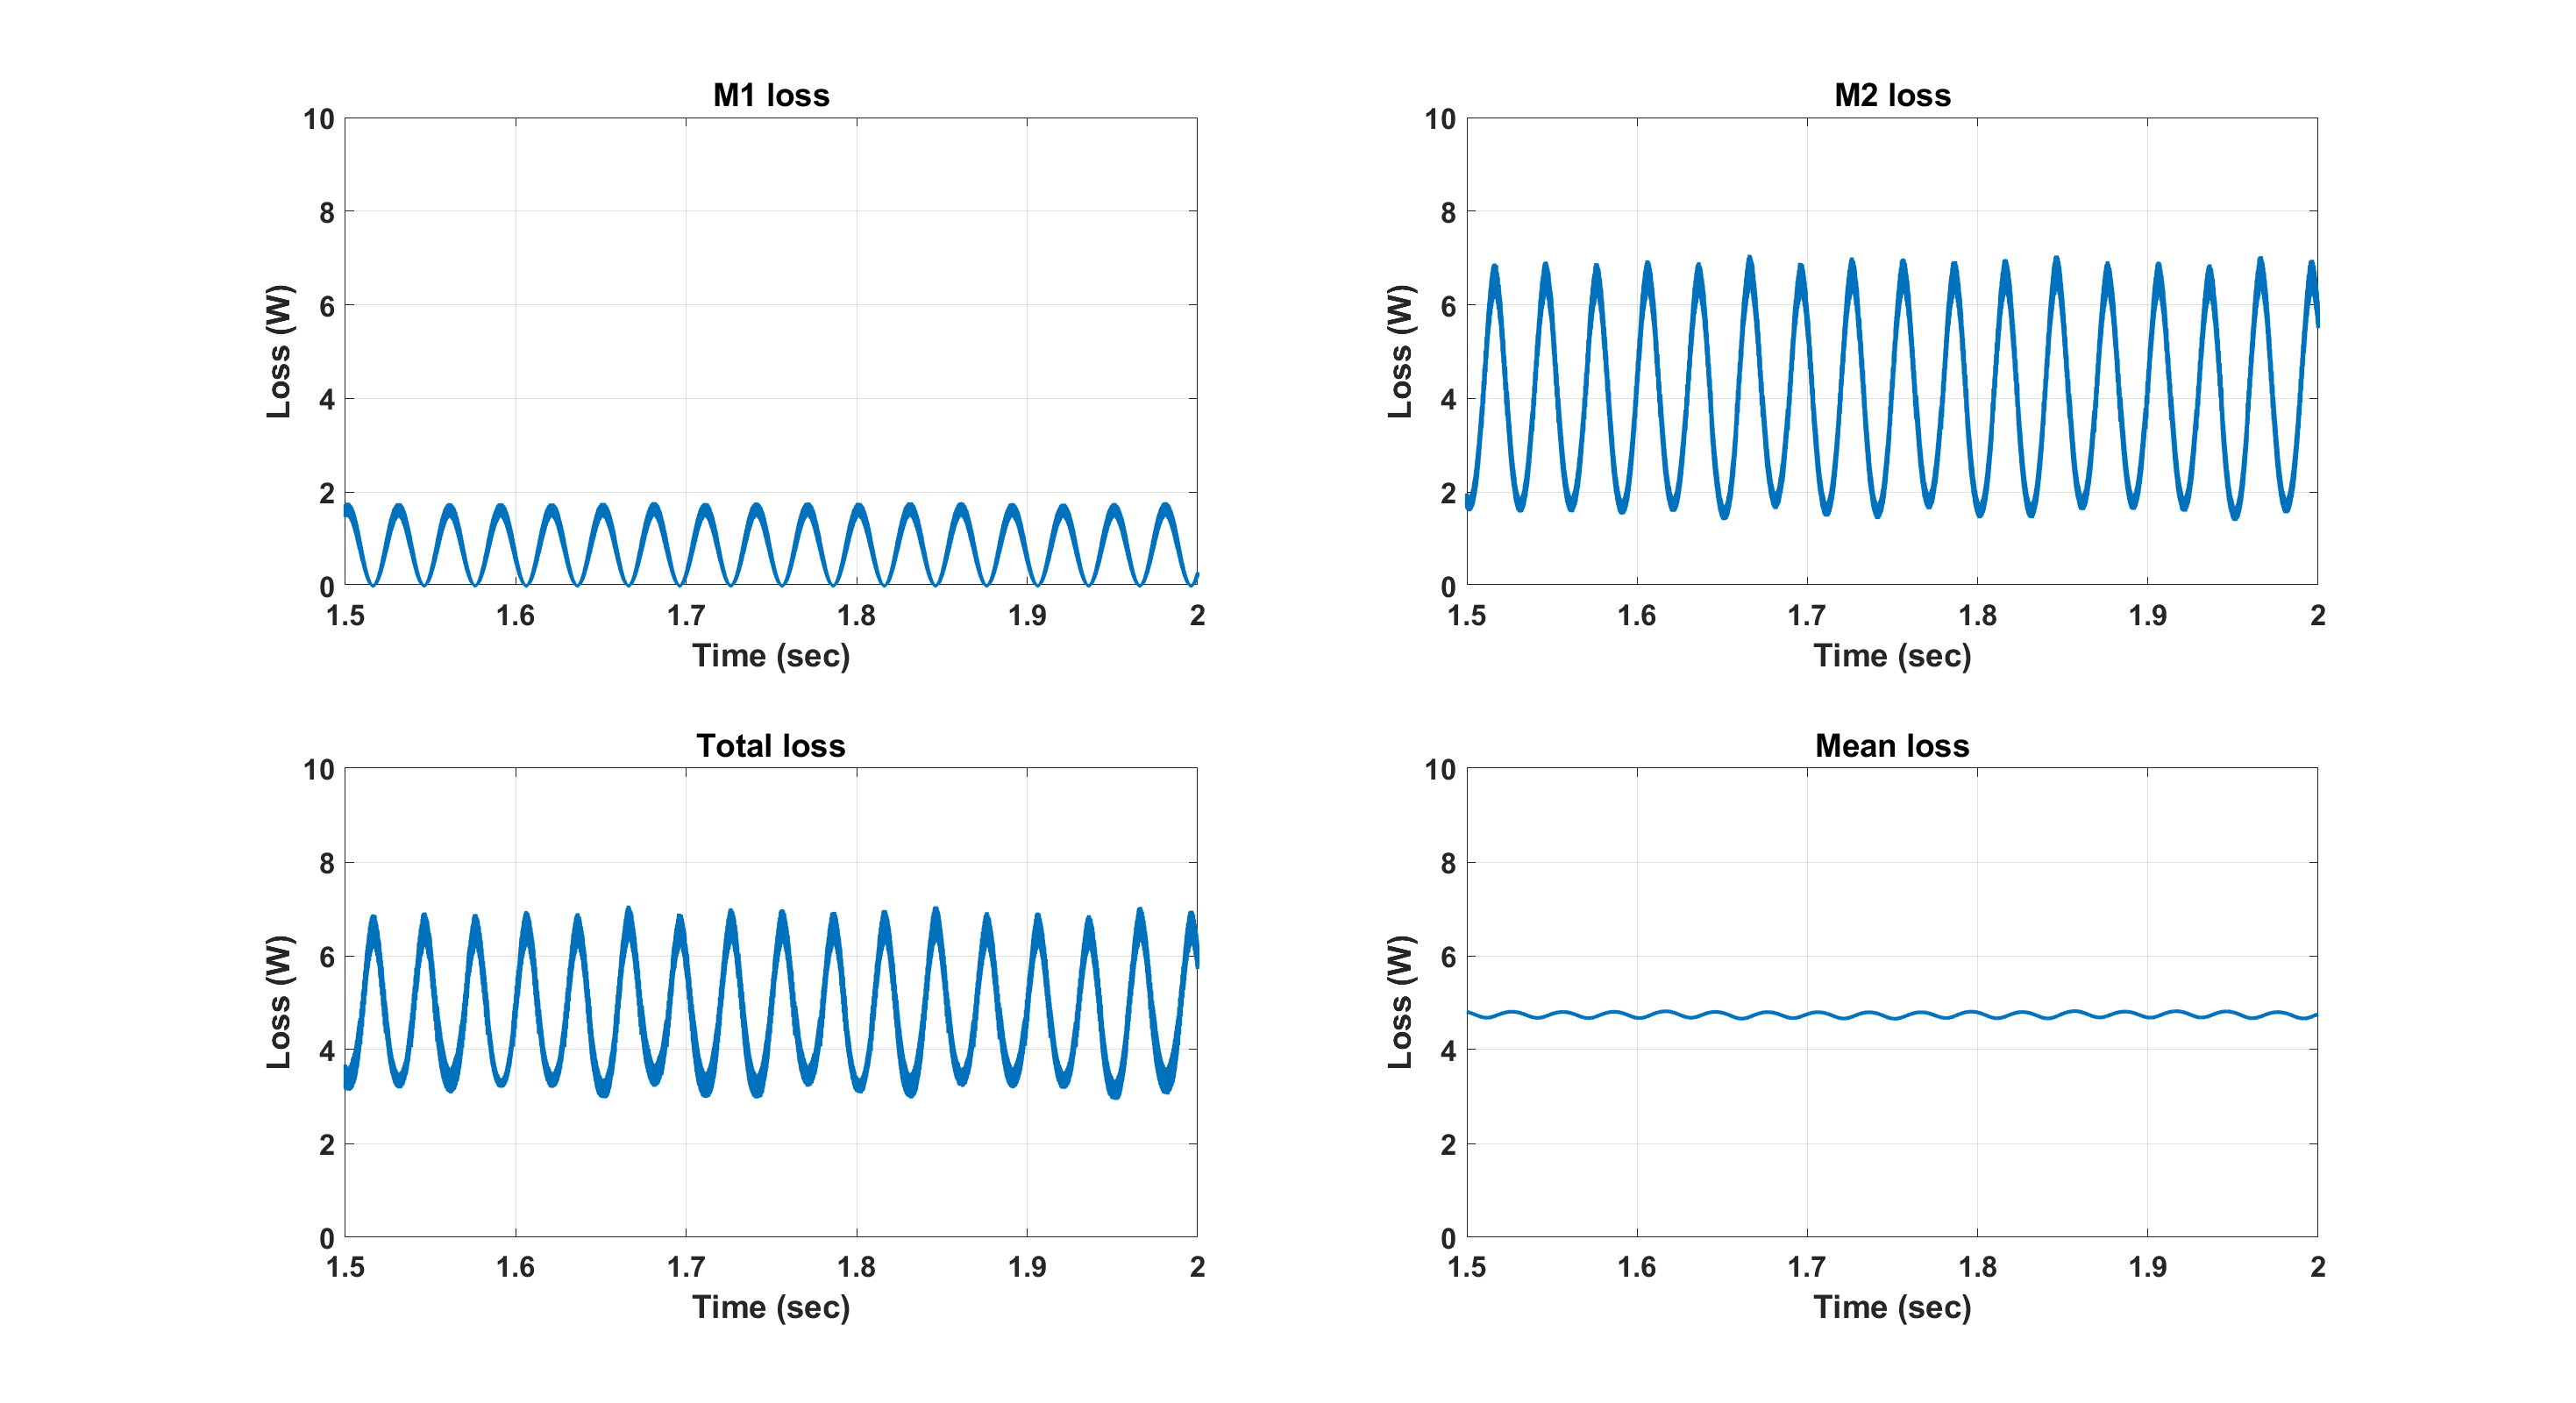
\includegraphics[scale=0.35]{SimulationResults/EqualTorqueShare/Loss_closer.eps}
\caption{Module Losses for Equal Torque Distribution Closer}
\label{fig:LossEqualCloser}
\end{figure}

\begin{figure}[H]
\centering
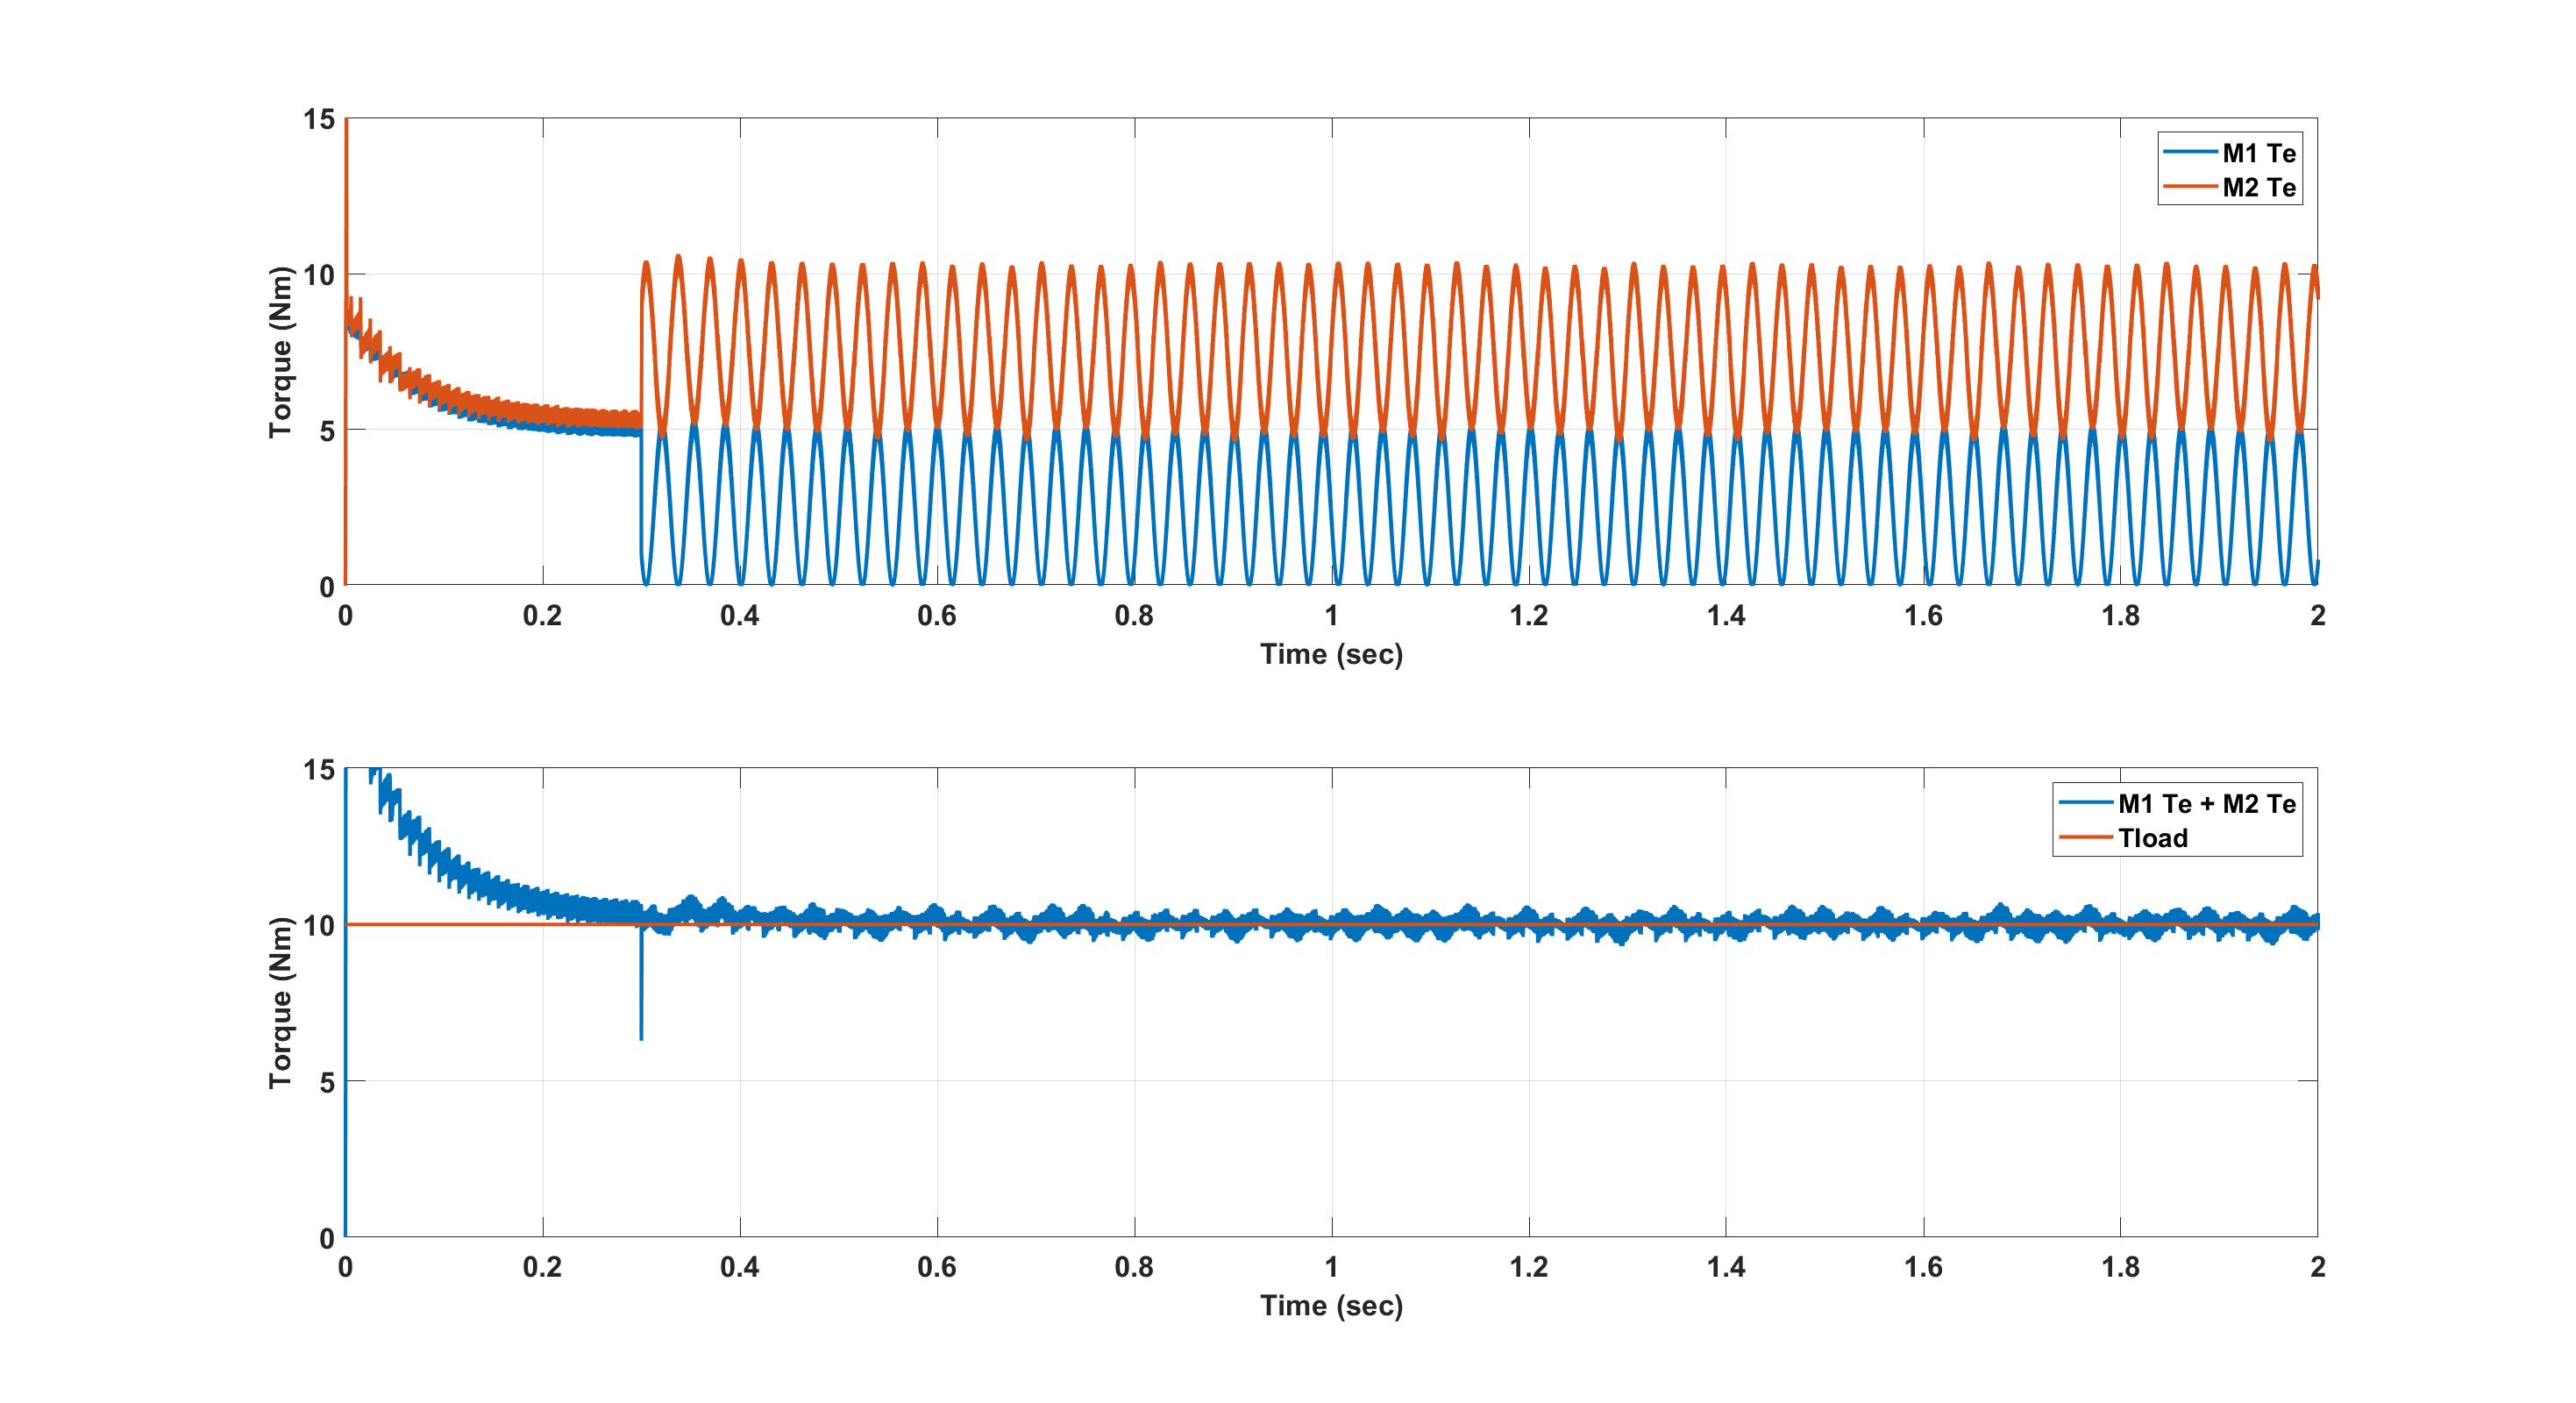
\includegraphics[scale=0.35]{SimulationResults/EqualTorqueShare/Torques.eps}
\caption{Module Losses for Equal Torque Distribution}
\label{fig:LossEqual}
\end{figure}

\section{Proposed Optimum on a paper}
\begin{figure}[H]
\centering
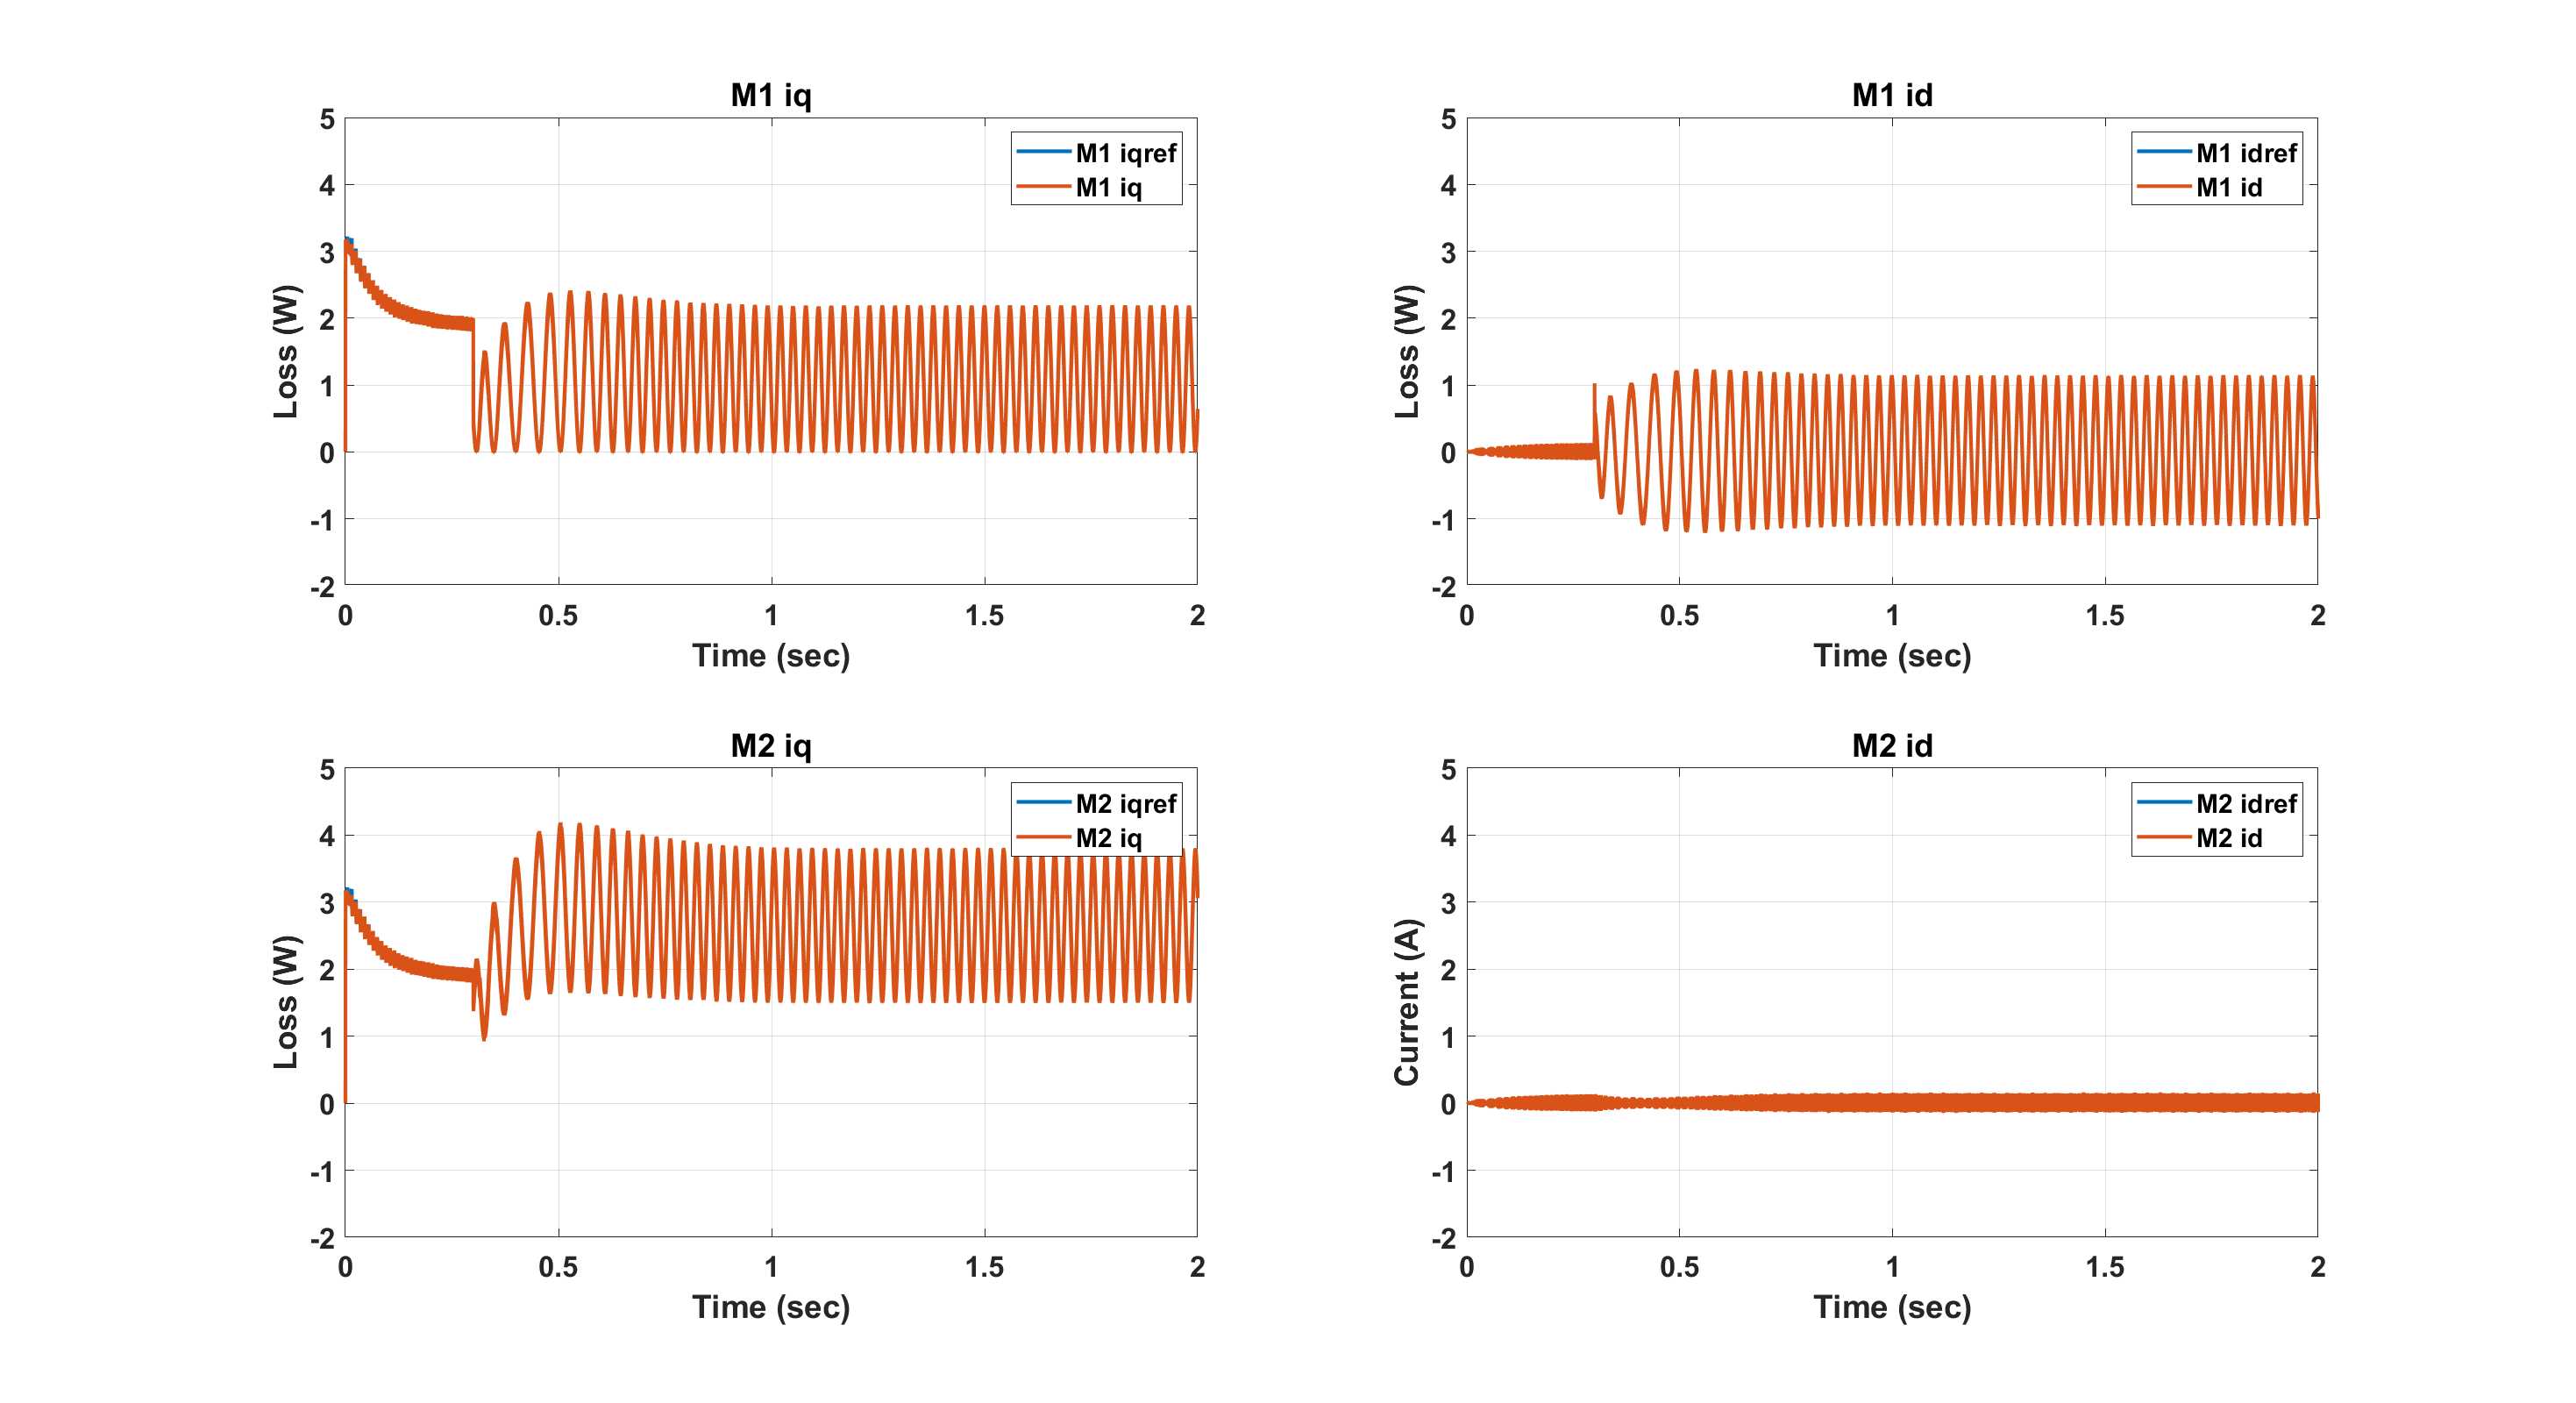
\includegraphics[scale=0.35]{SimulationResults/ProposedOptimum/idq_refs.eps}
\caption{dq Phase Currents and References for Proposed Optimum Distribution}
\label{fig:PhaseCurrentsReferencesProposedOptimum}
\end{figure}

\begin{figure}[H]
\centering
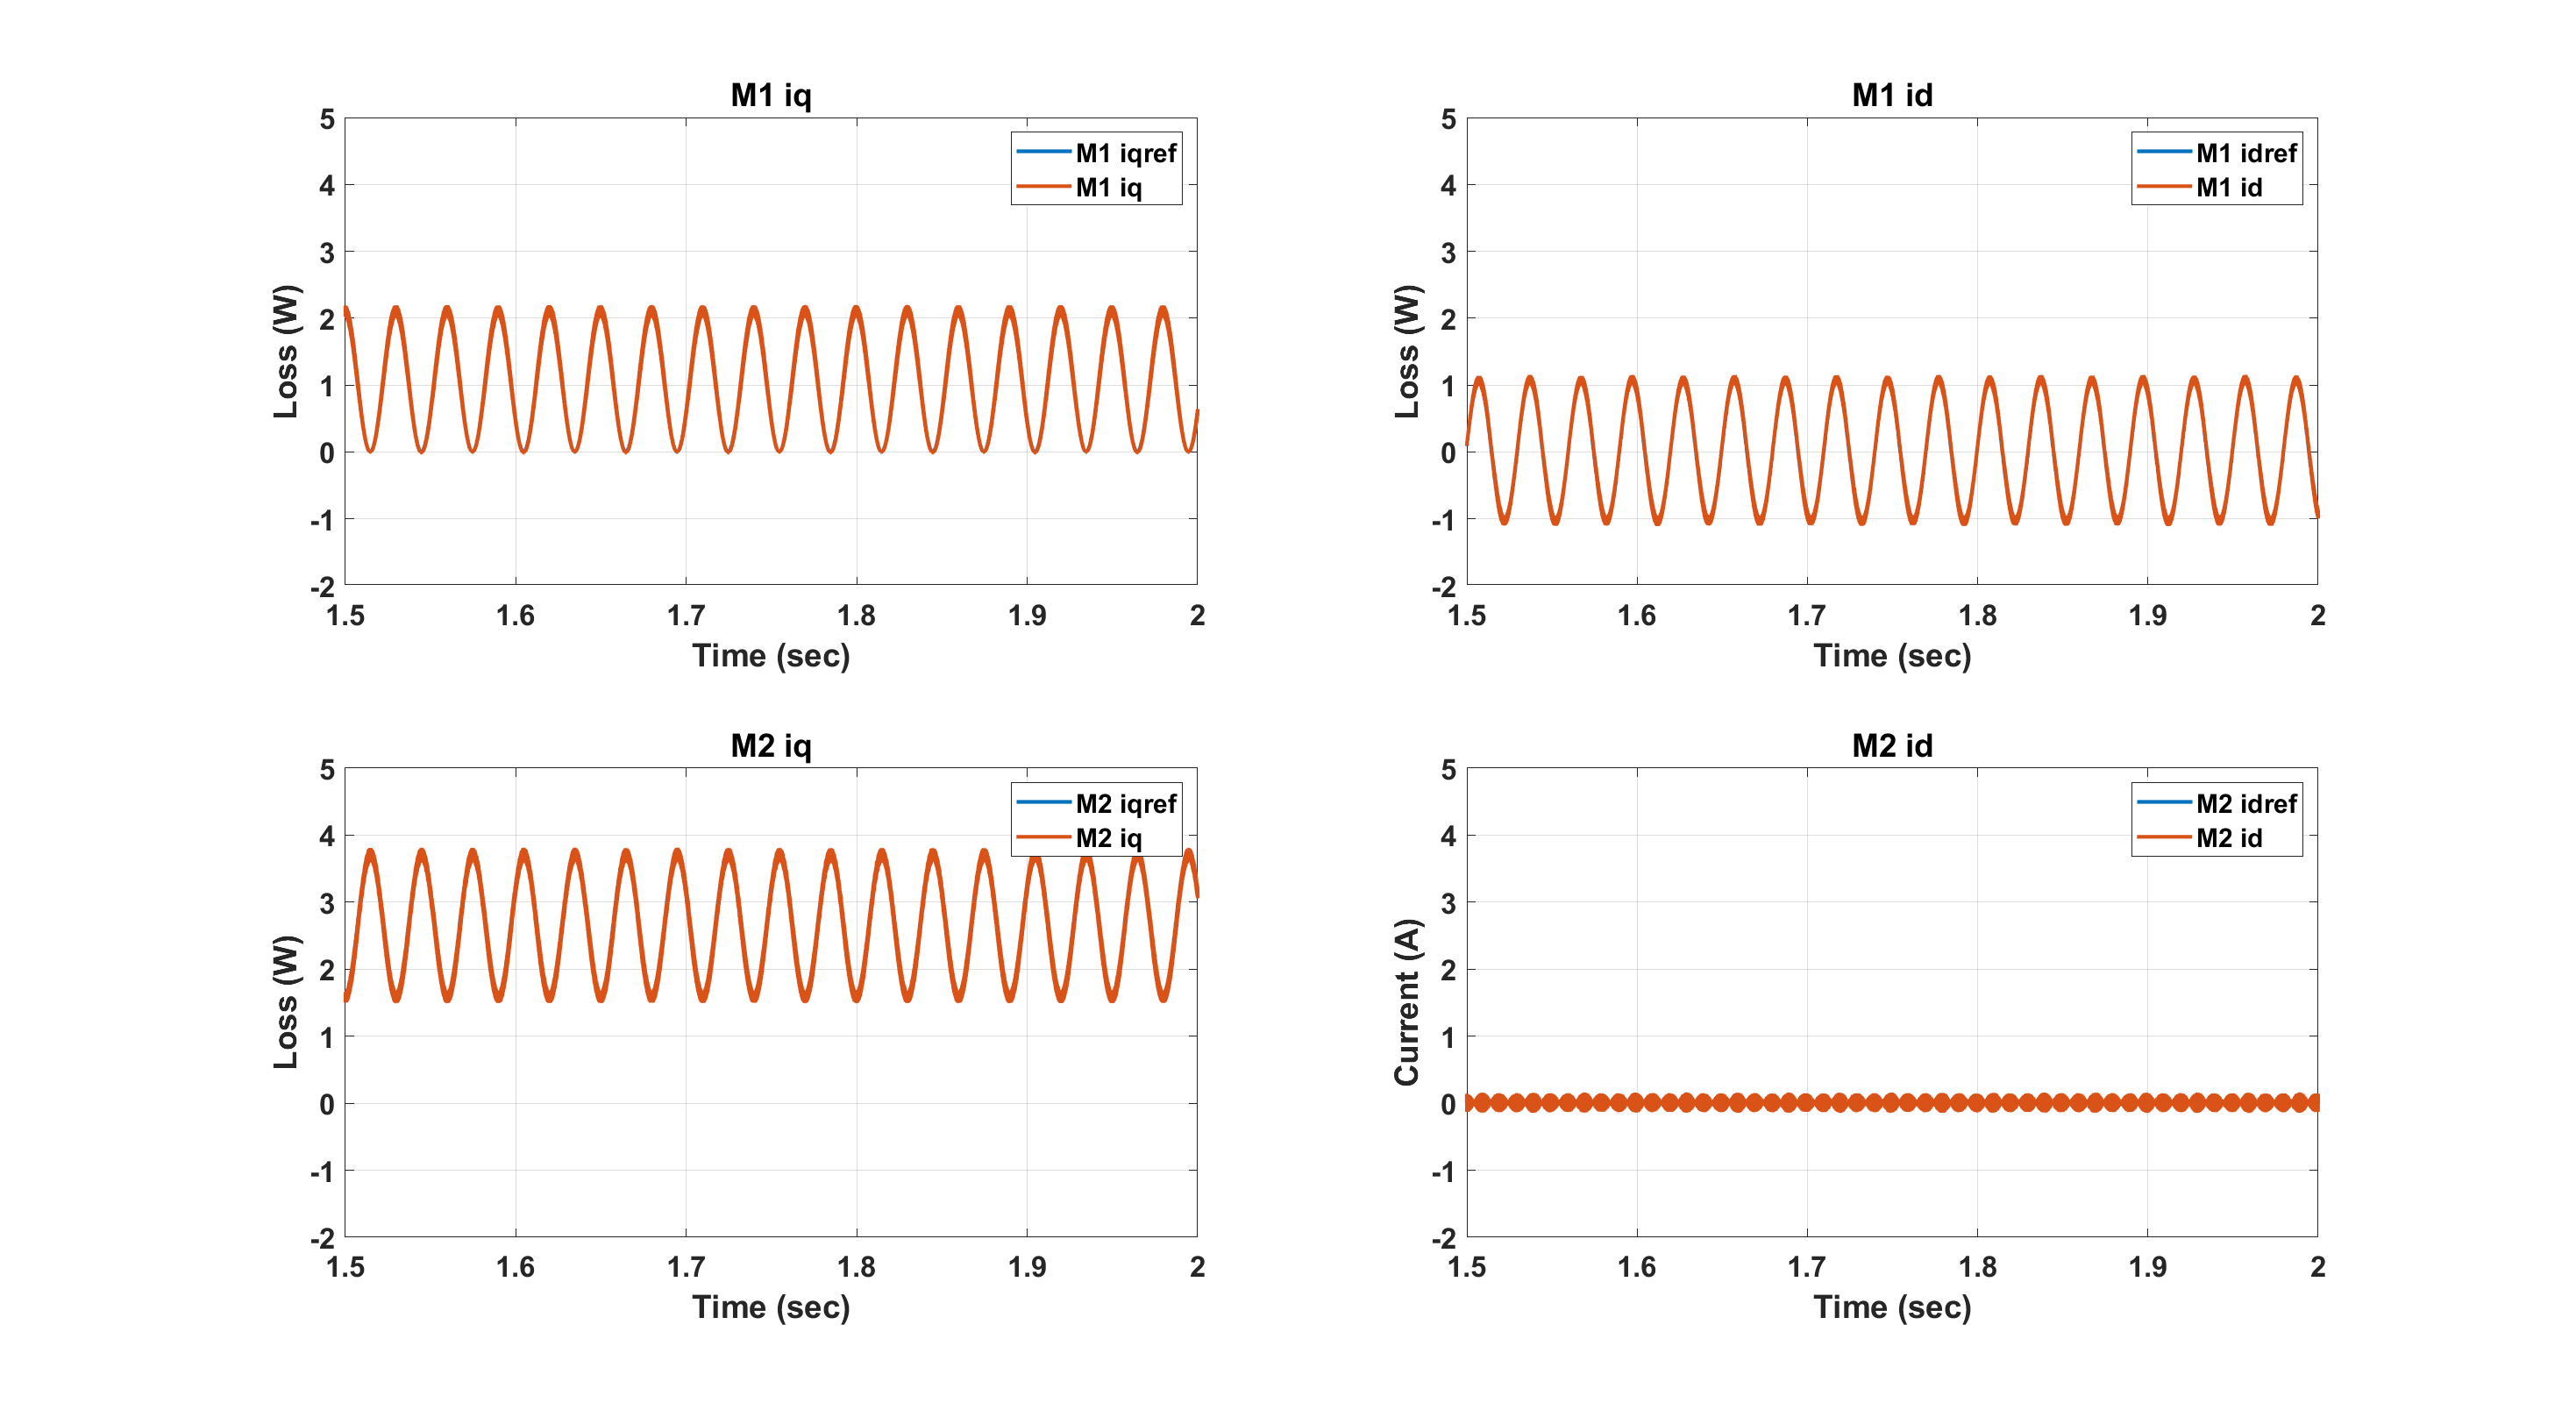
\includegraphics[scale=0.35]{SimulationResults/ProposedOptimum/idq_refs_closer.eps}
\caption{dq Phase Currents and References for Proposed Optimum Distribution Closer}
\label{fig:PhaseCurrentsReferencesProposedOptimumCloser}
\end{figure}

\begin{figure}[H]
\centering
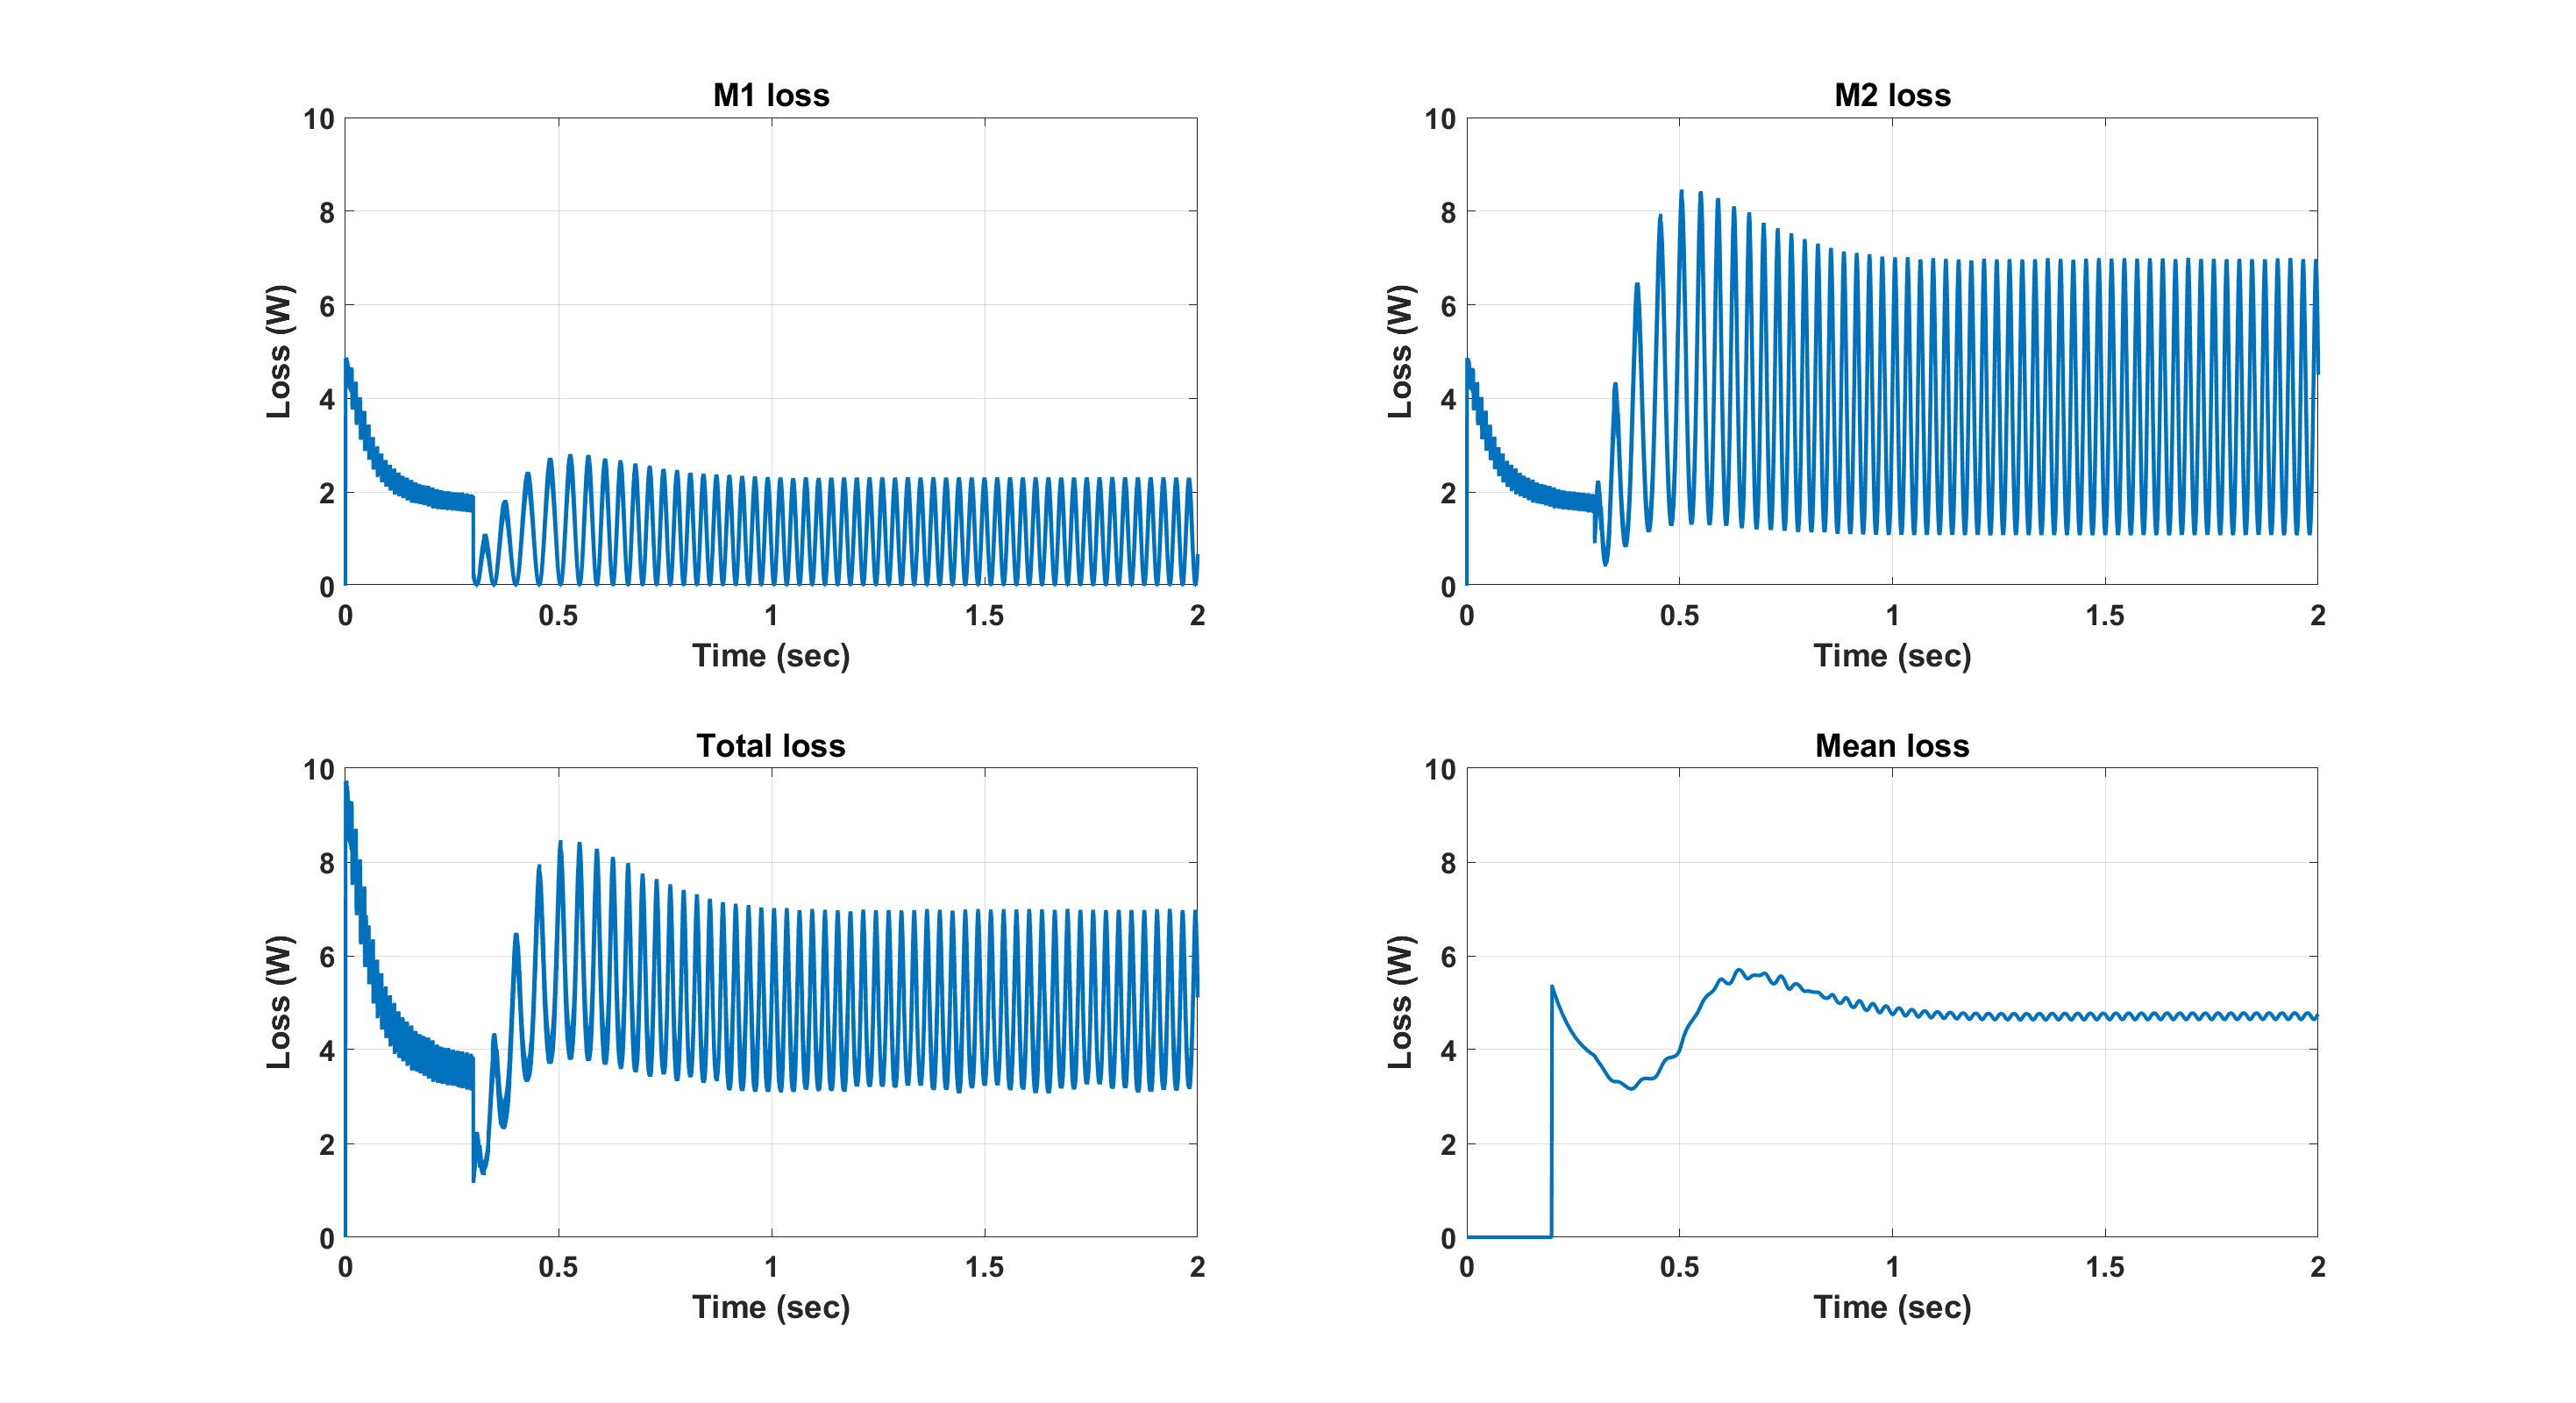
\includegraphics[scale=0.35]{SimulationResults/ProposedOptimum/Loss.eps}
\caption{Module Losses for Proposed Optimum Distribution}
\label{fig:LossProposedOptimum}
\end{figure}

\begin{figure}[H]
\centering
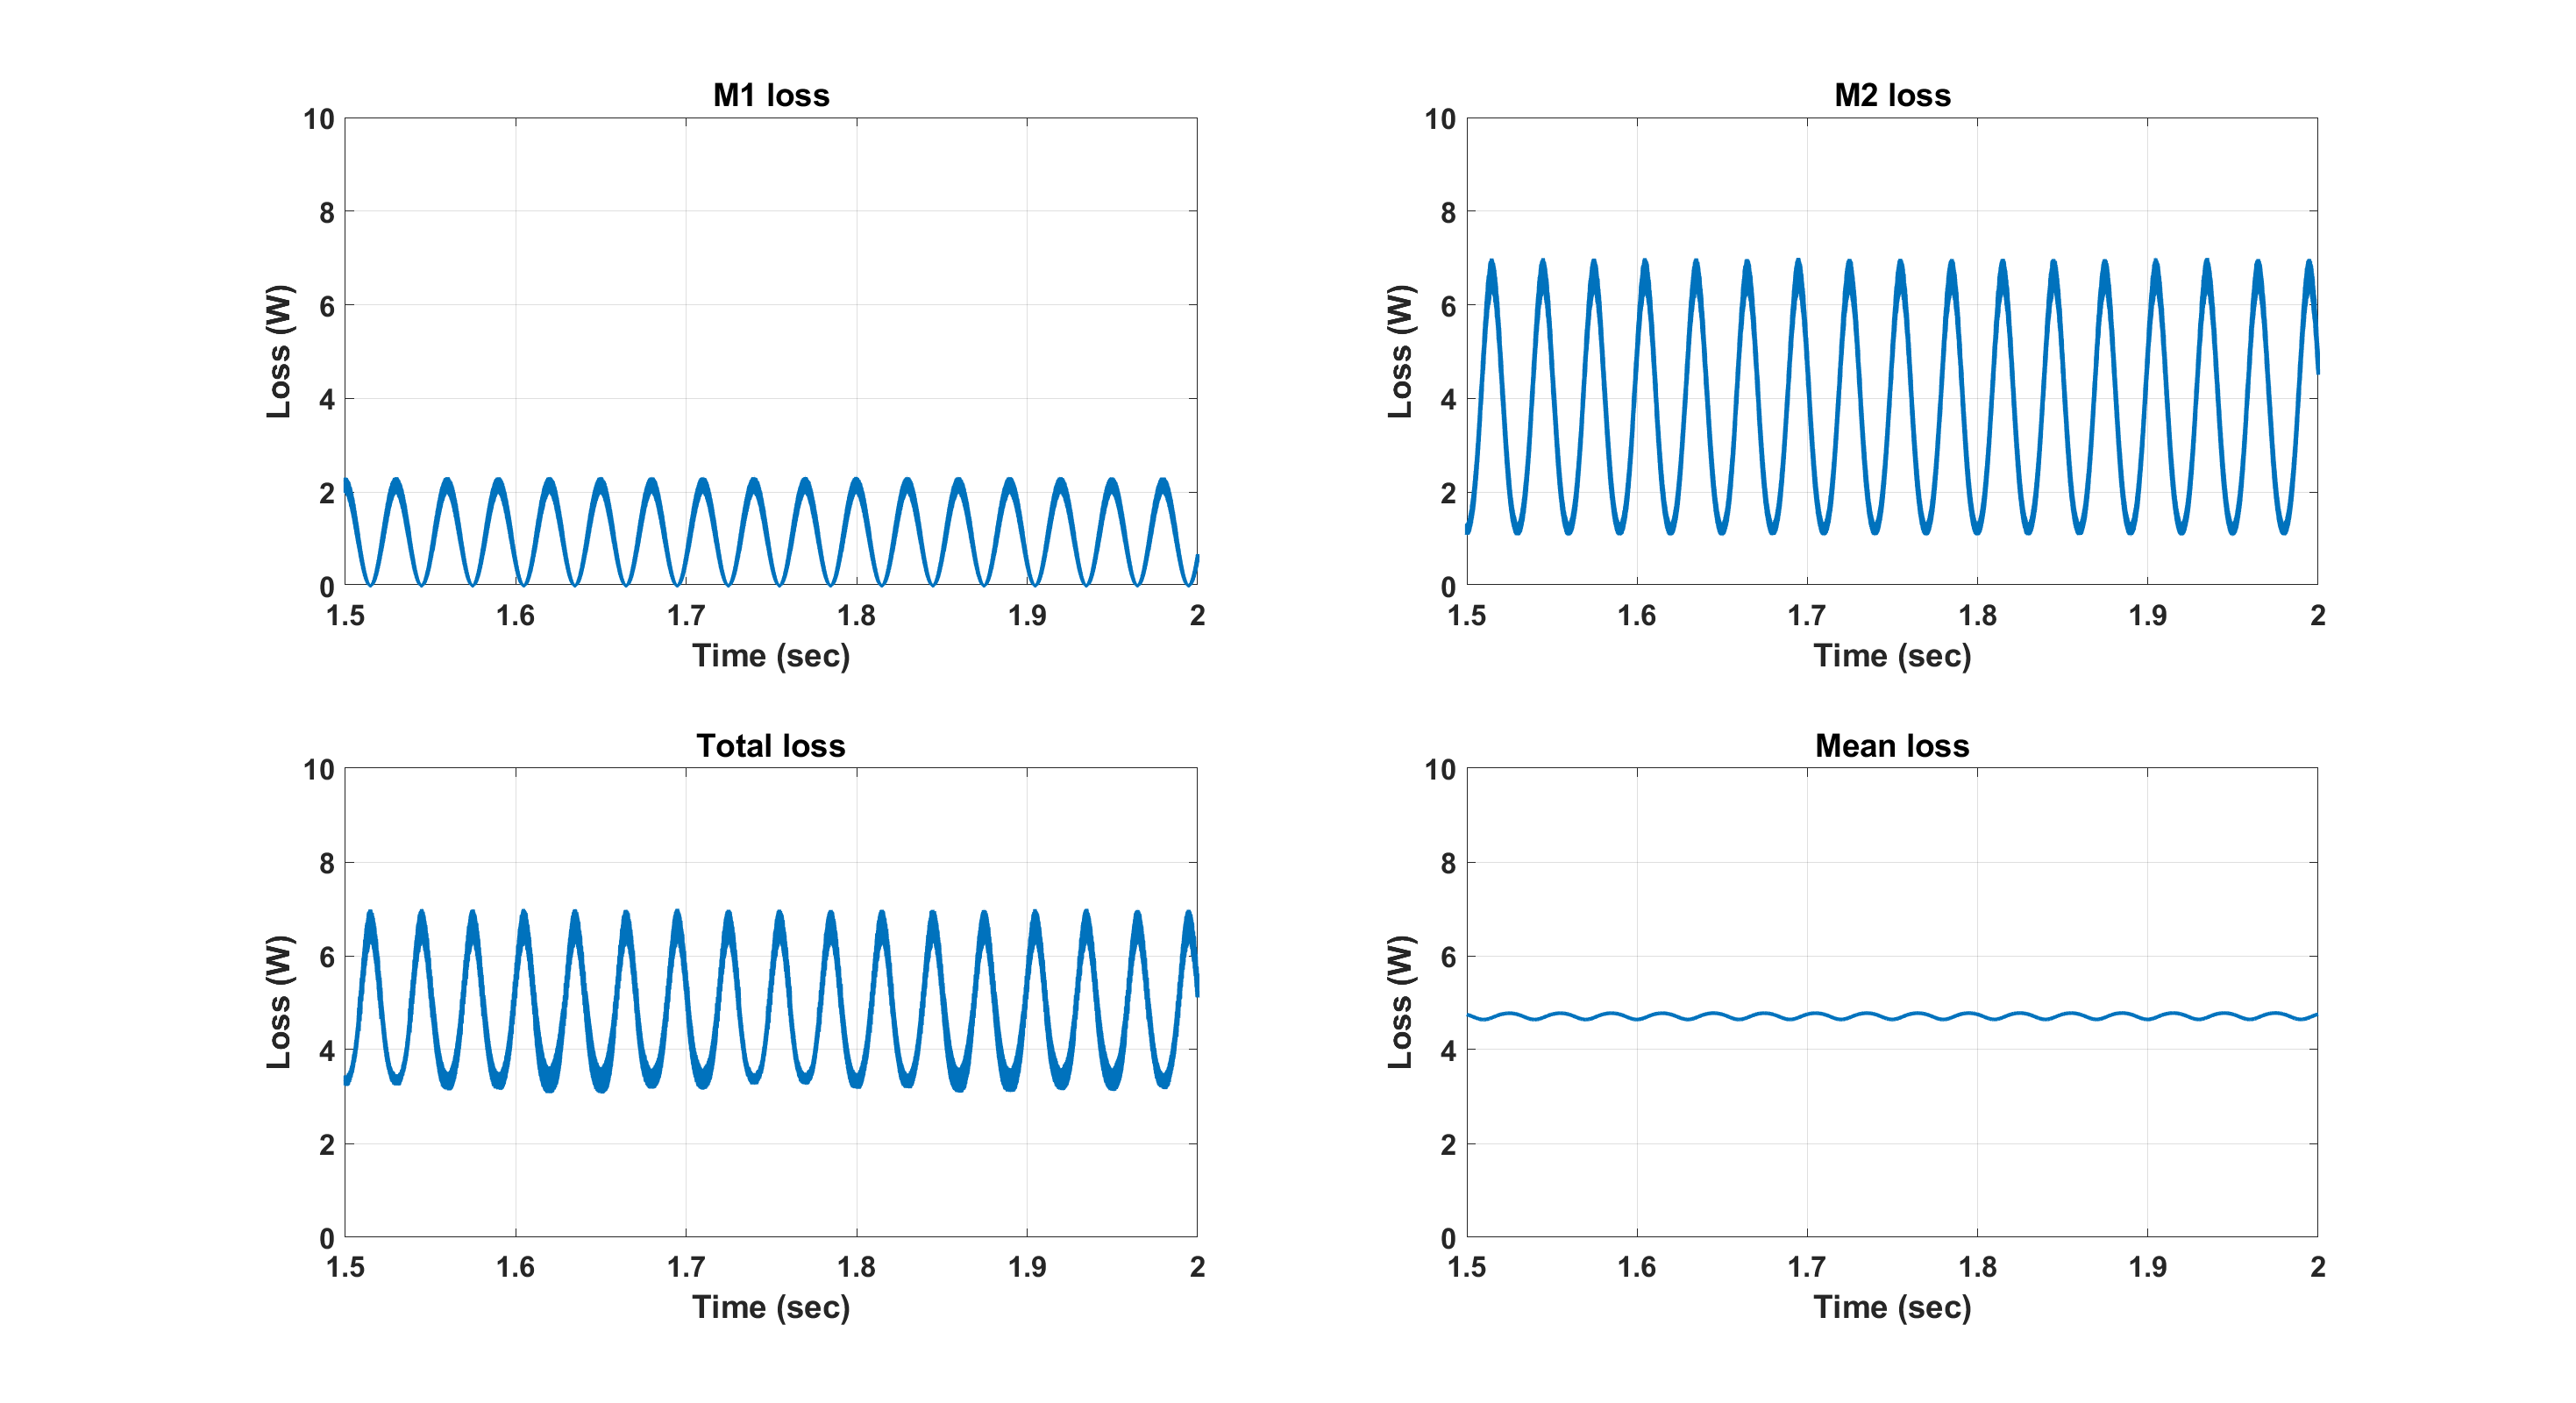
\includegraphics[scale=0.35]{SimulationResults/ProposedOptimum/Loss_closer.eps}
\caption{Module Losses for Proposed Optimum Distribution Closer}
\label{fig:LossProposedOptimumCloser}
\end{figure}

\begin{figure}[H]
\centering
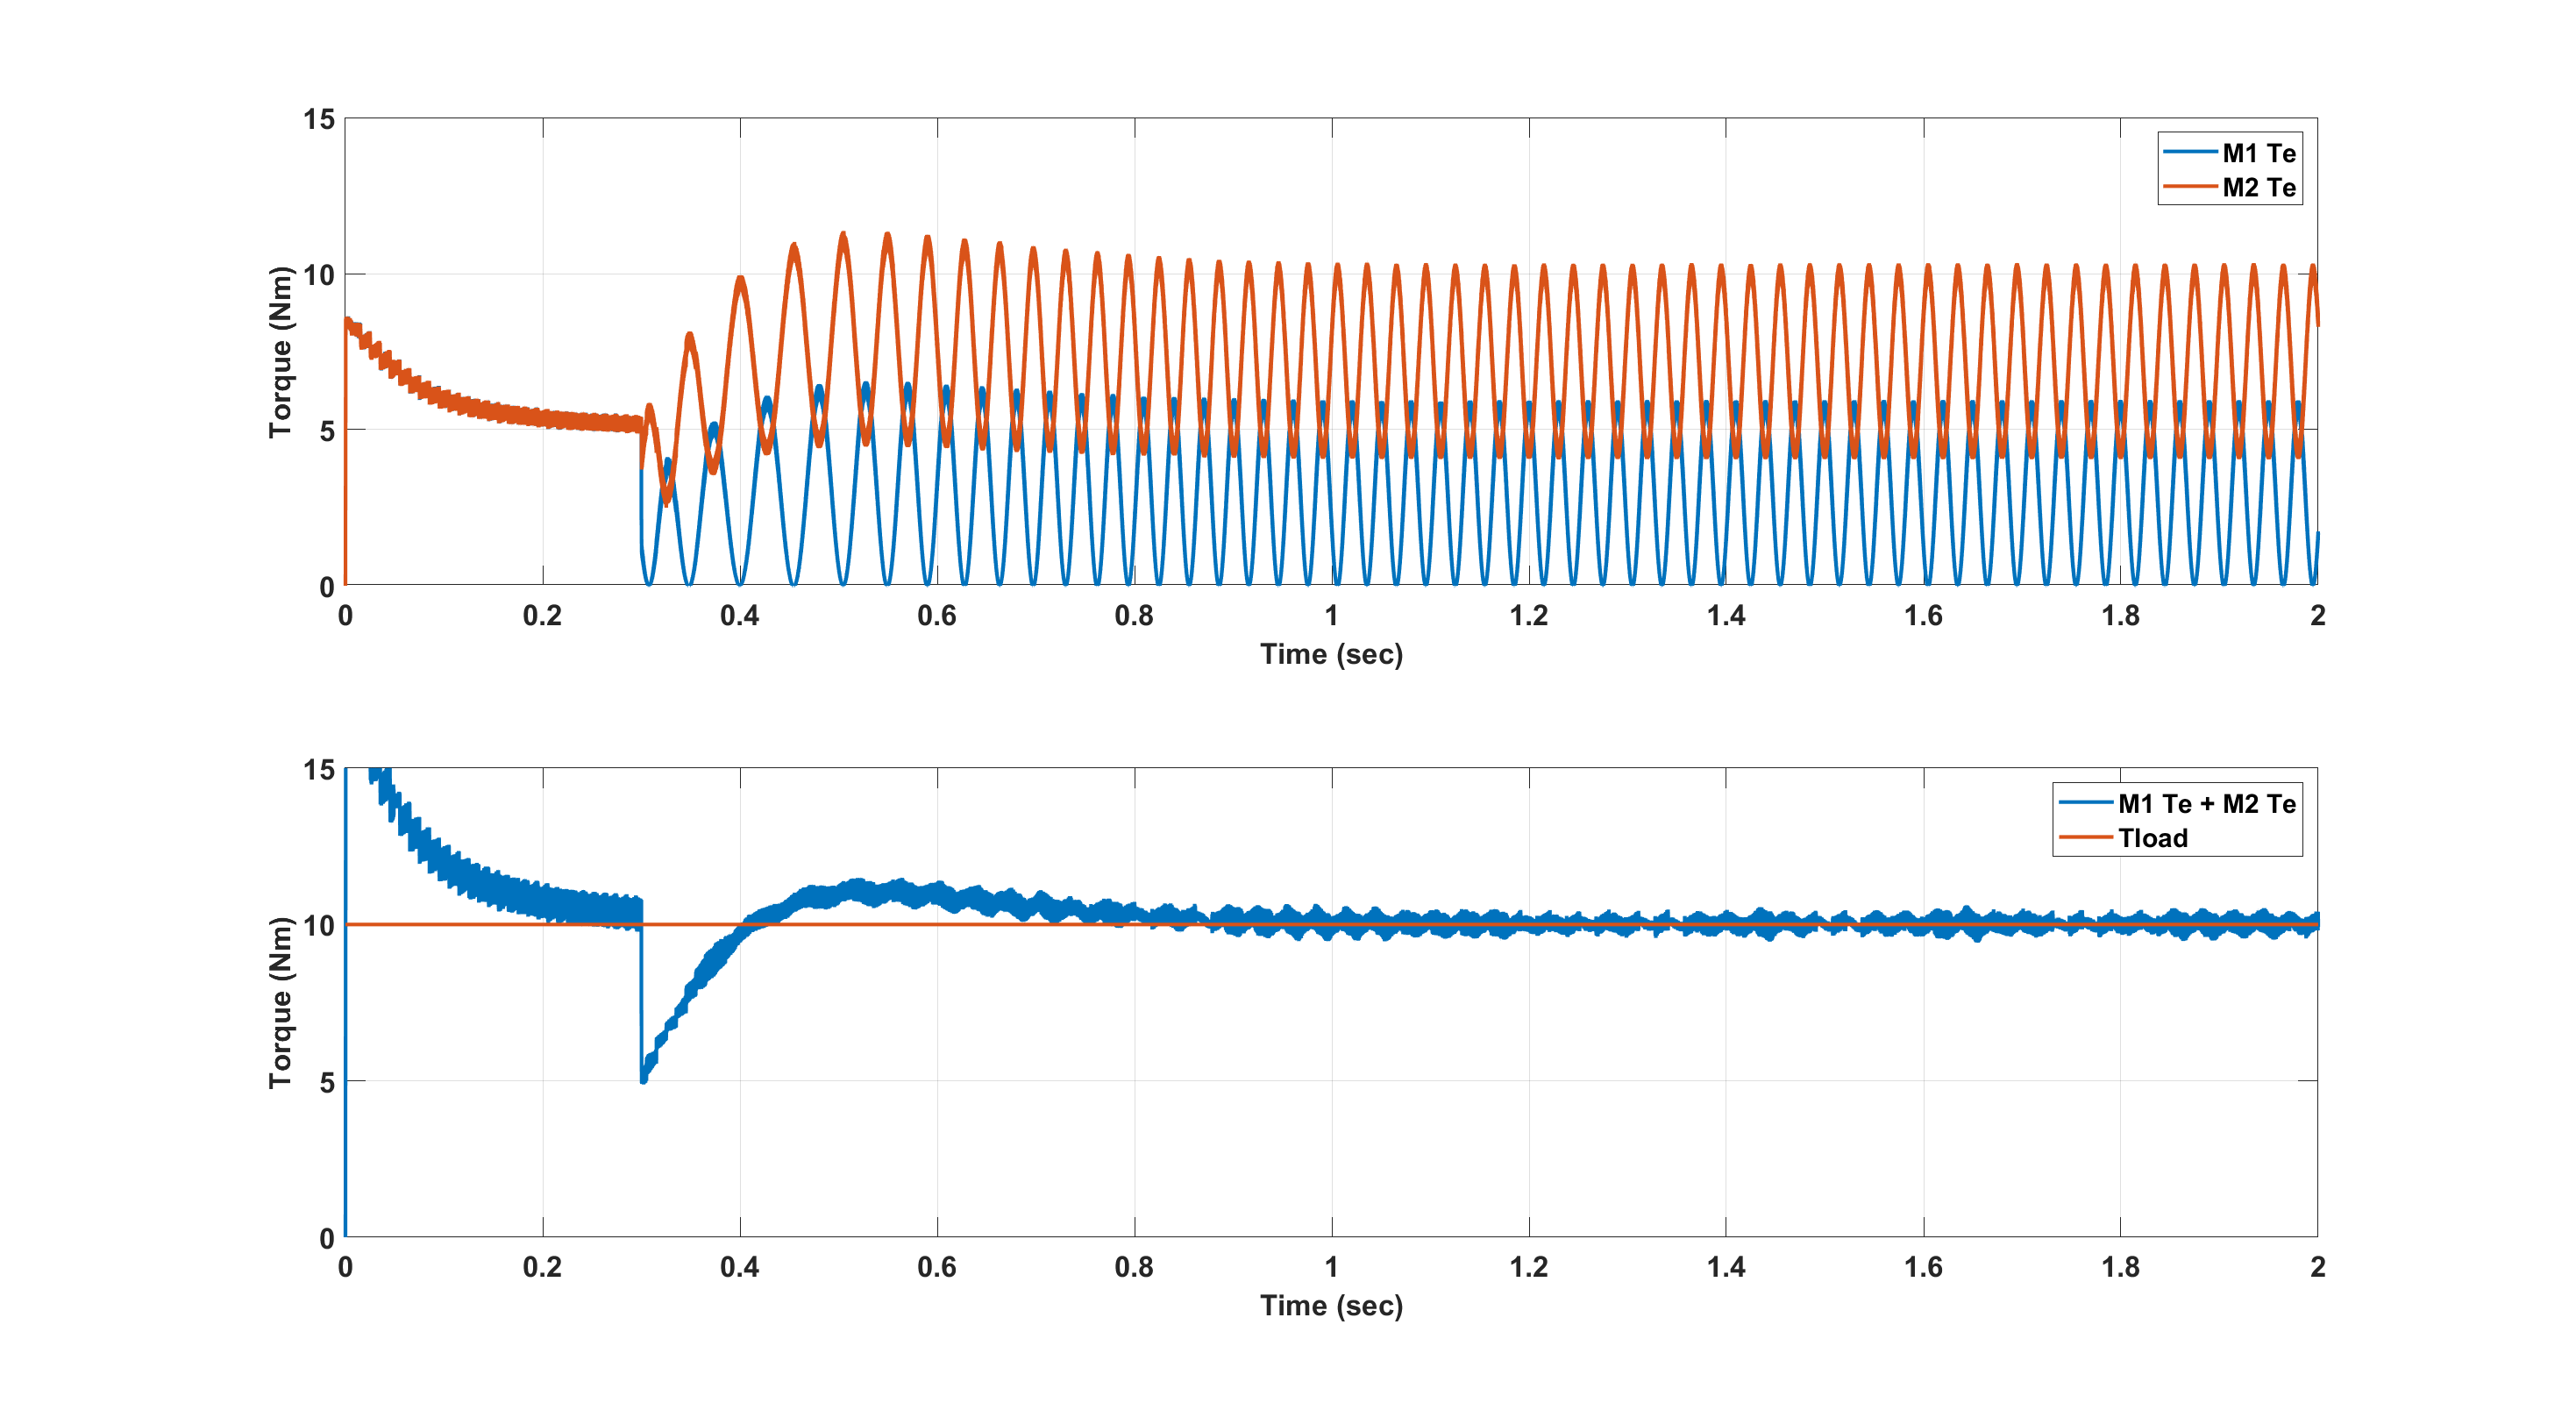
\includegraphics[scale=0.35]{SimulationResults/ProposedOptimum/Torques.eps}
\caption{Module Losses for Proposed Optimum Distribution}
\label{fig:LossProposedOptimum}
\end{figure}


\section{MyMethod}
\begin{figure}[H]
\centering
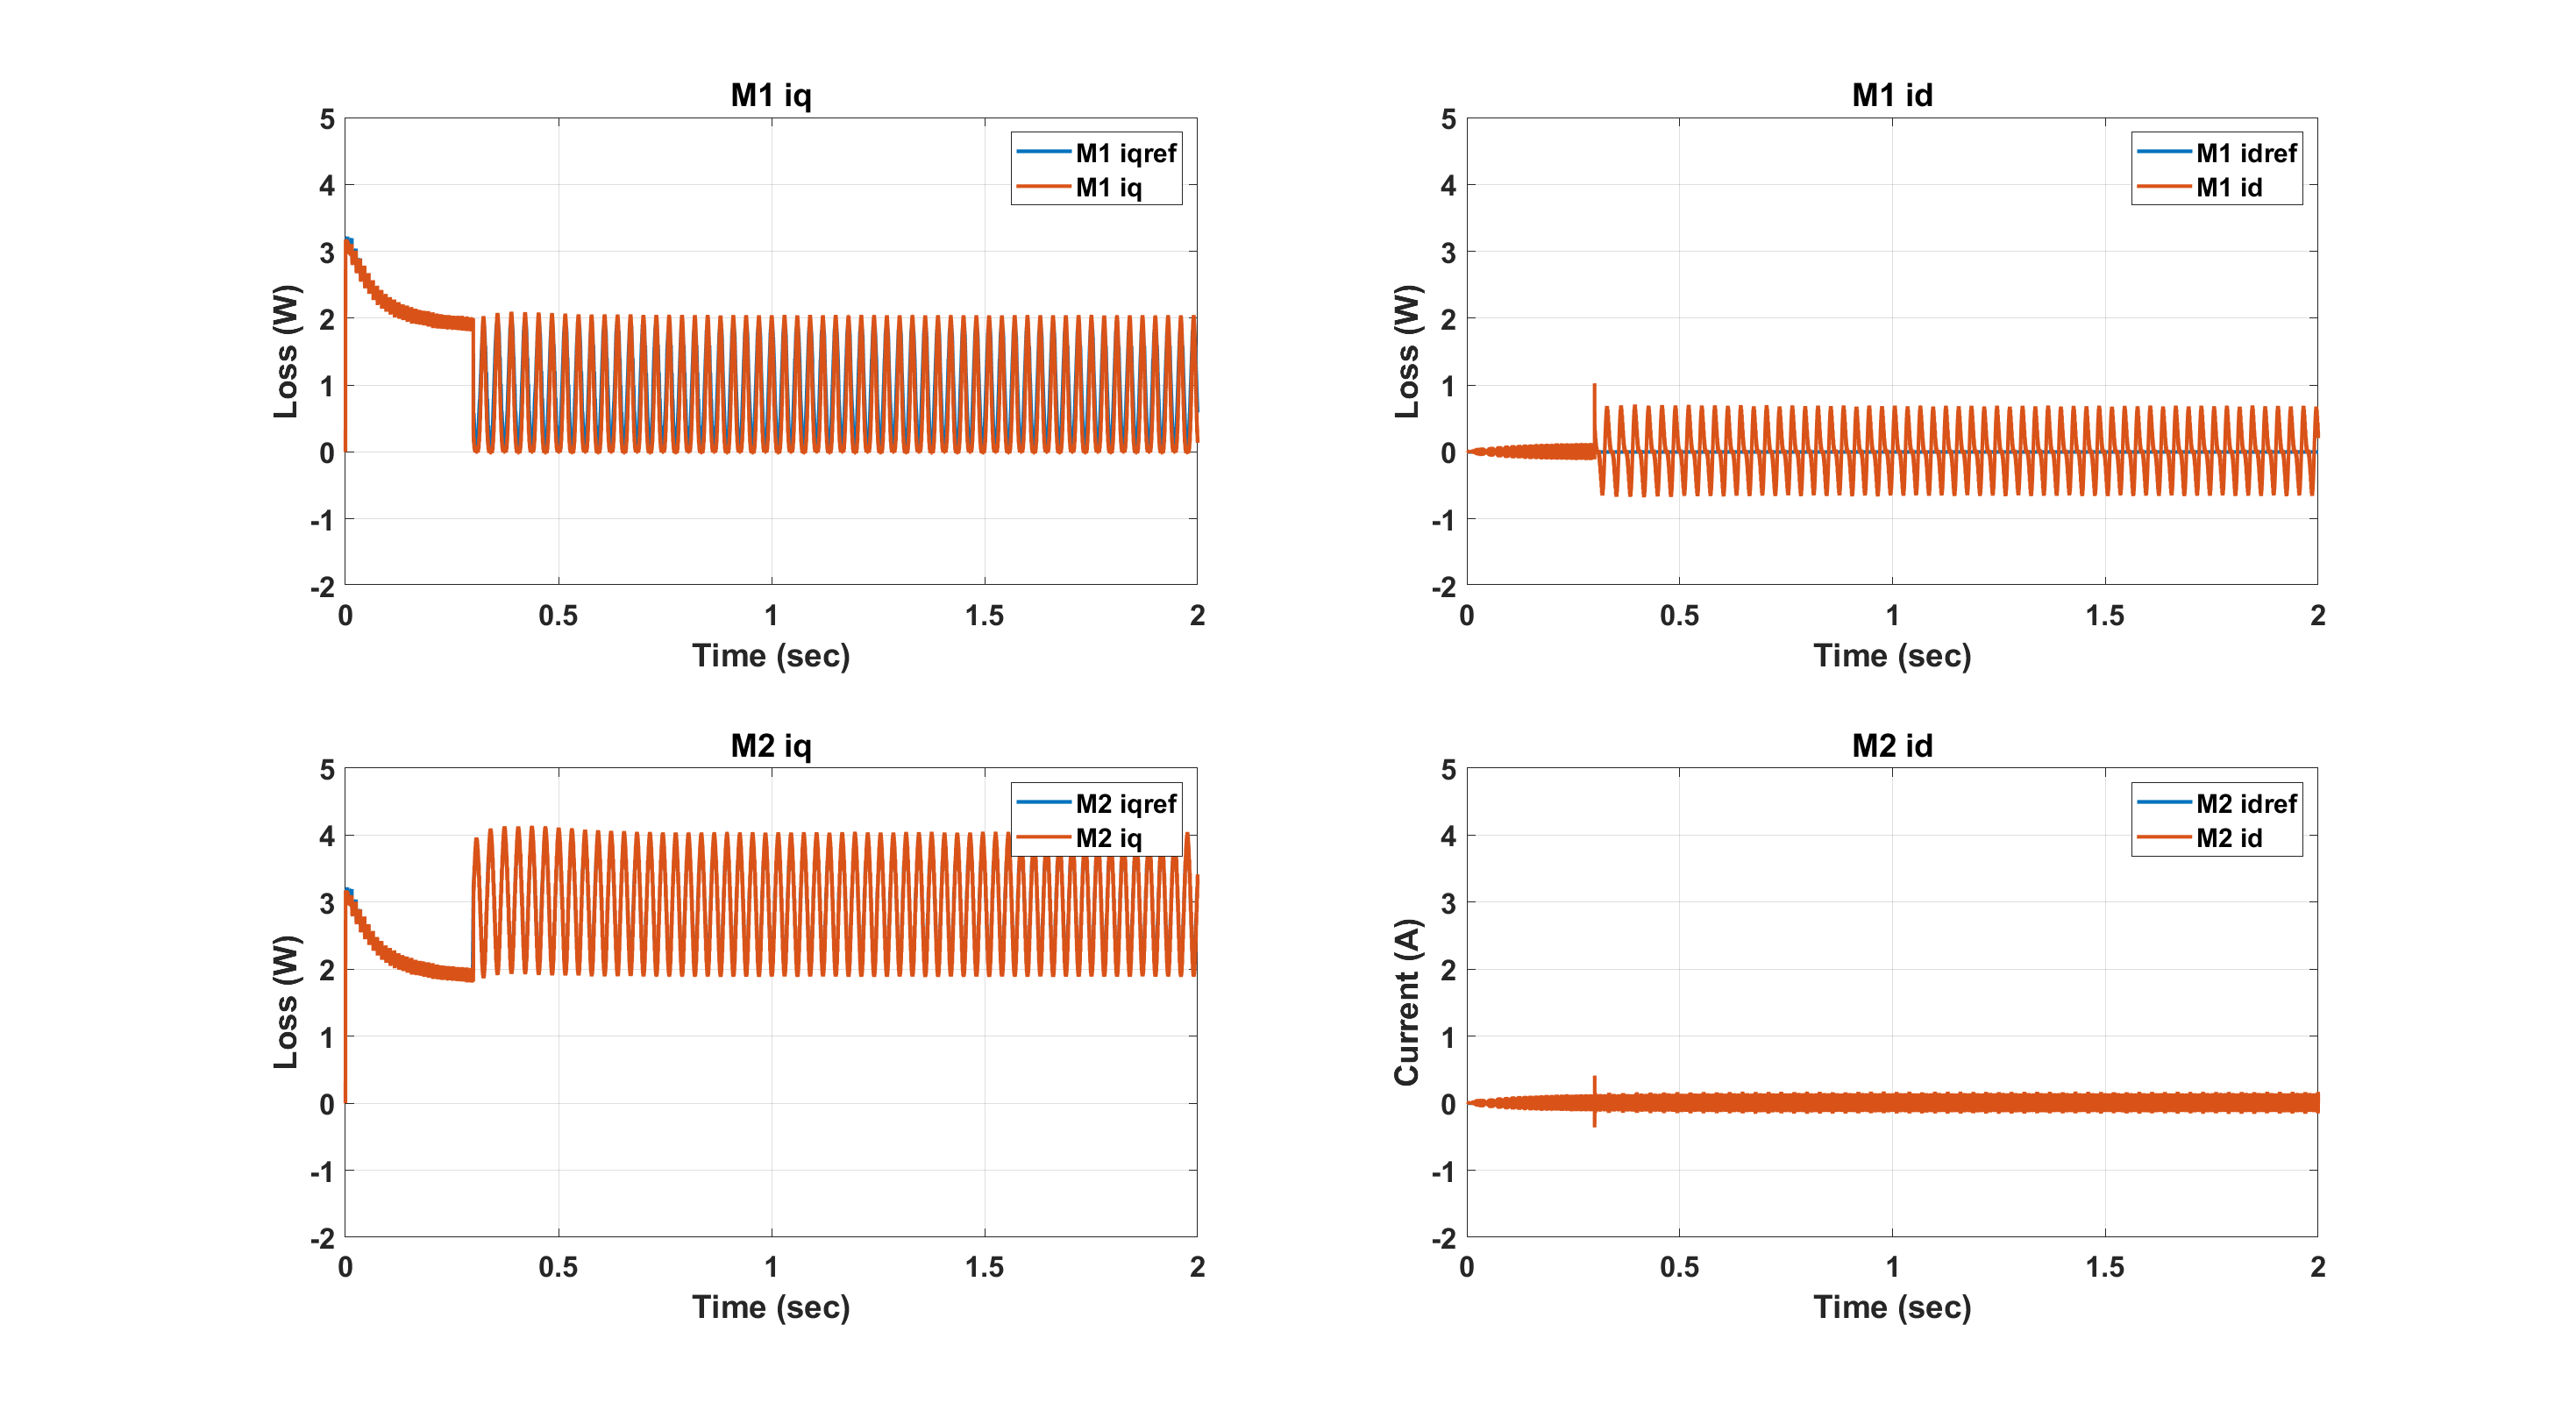
\includegraphics[scale=0.35]{SimulationResults/MyMethod/idq_refs.eps}
\caption{dq Phase Currents and References for My Method}
\label{fig:PhaseCurrentsReferencesMyMethod}
\end{figure}

\begin{figure}[H]
\centering
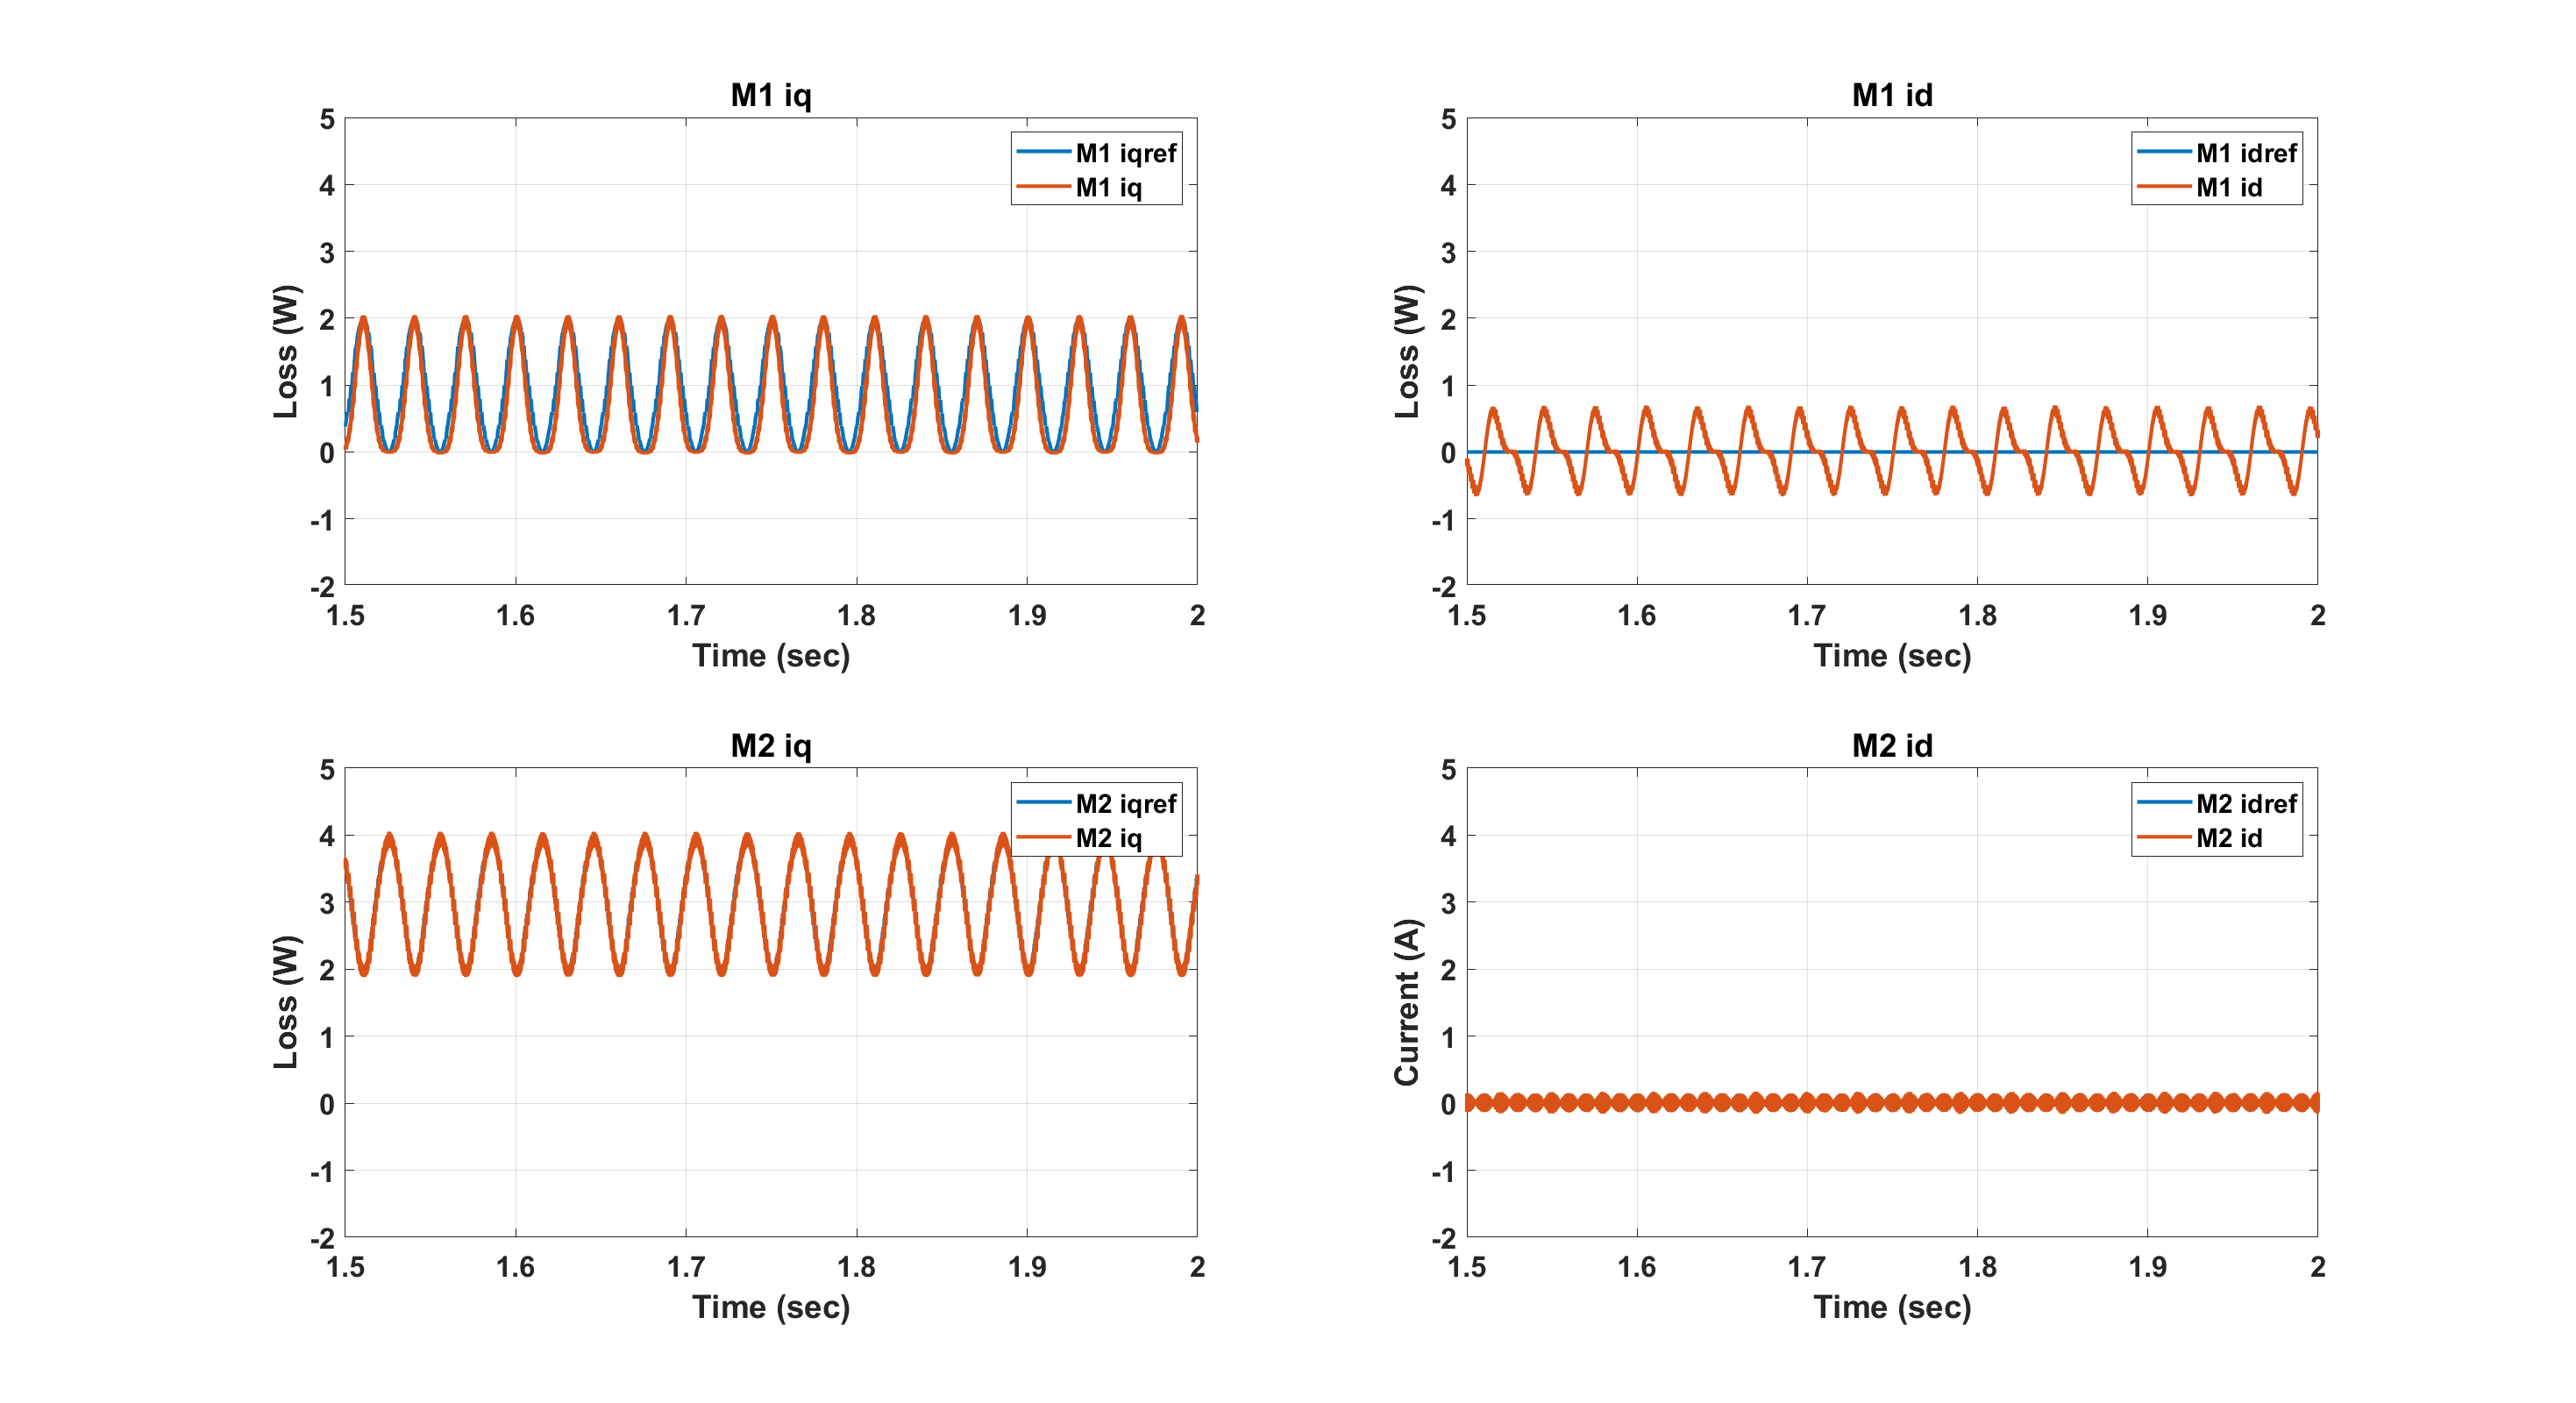
\includegraphics[scale=0.35]{SimulationResults/MyMethod/idq_refs_closer.eps}
\caption{dq Phase Currents and References for My Method Closer}
\label{fig:PhaseCurrentsReferencesMyMethodCloser}
\end{figure}

\begin{figure}[H]
\centering
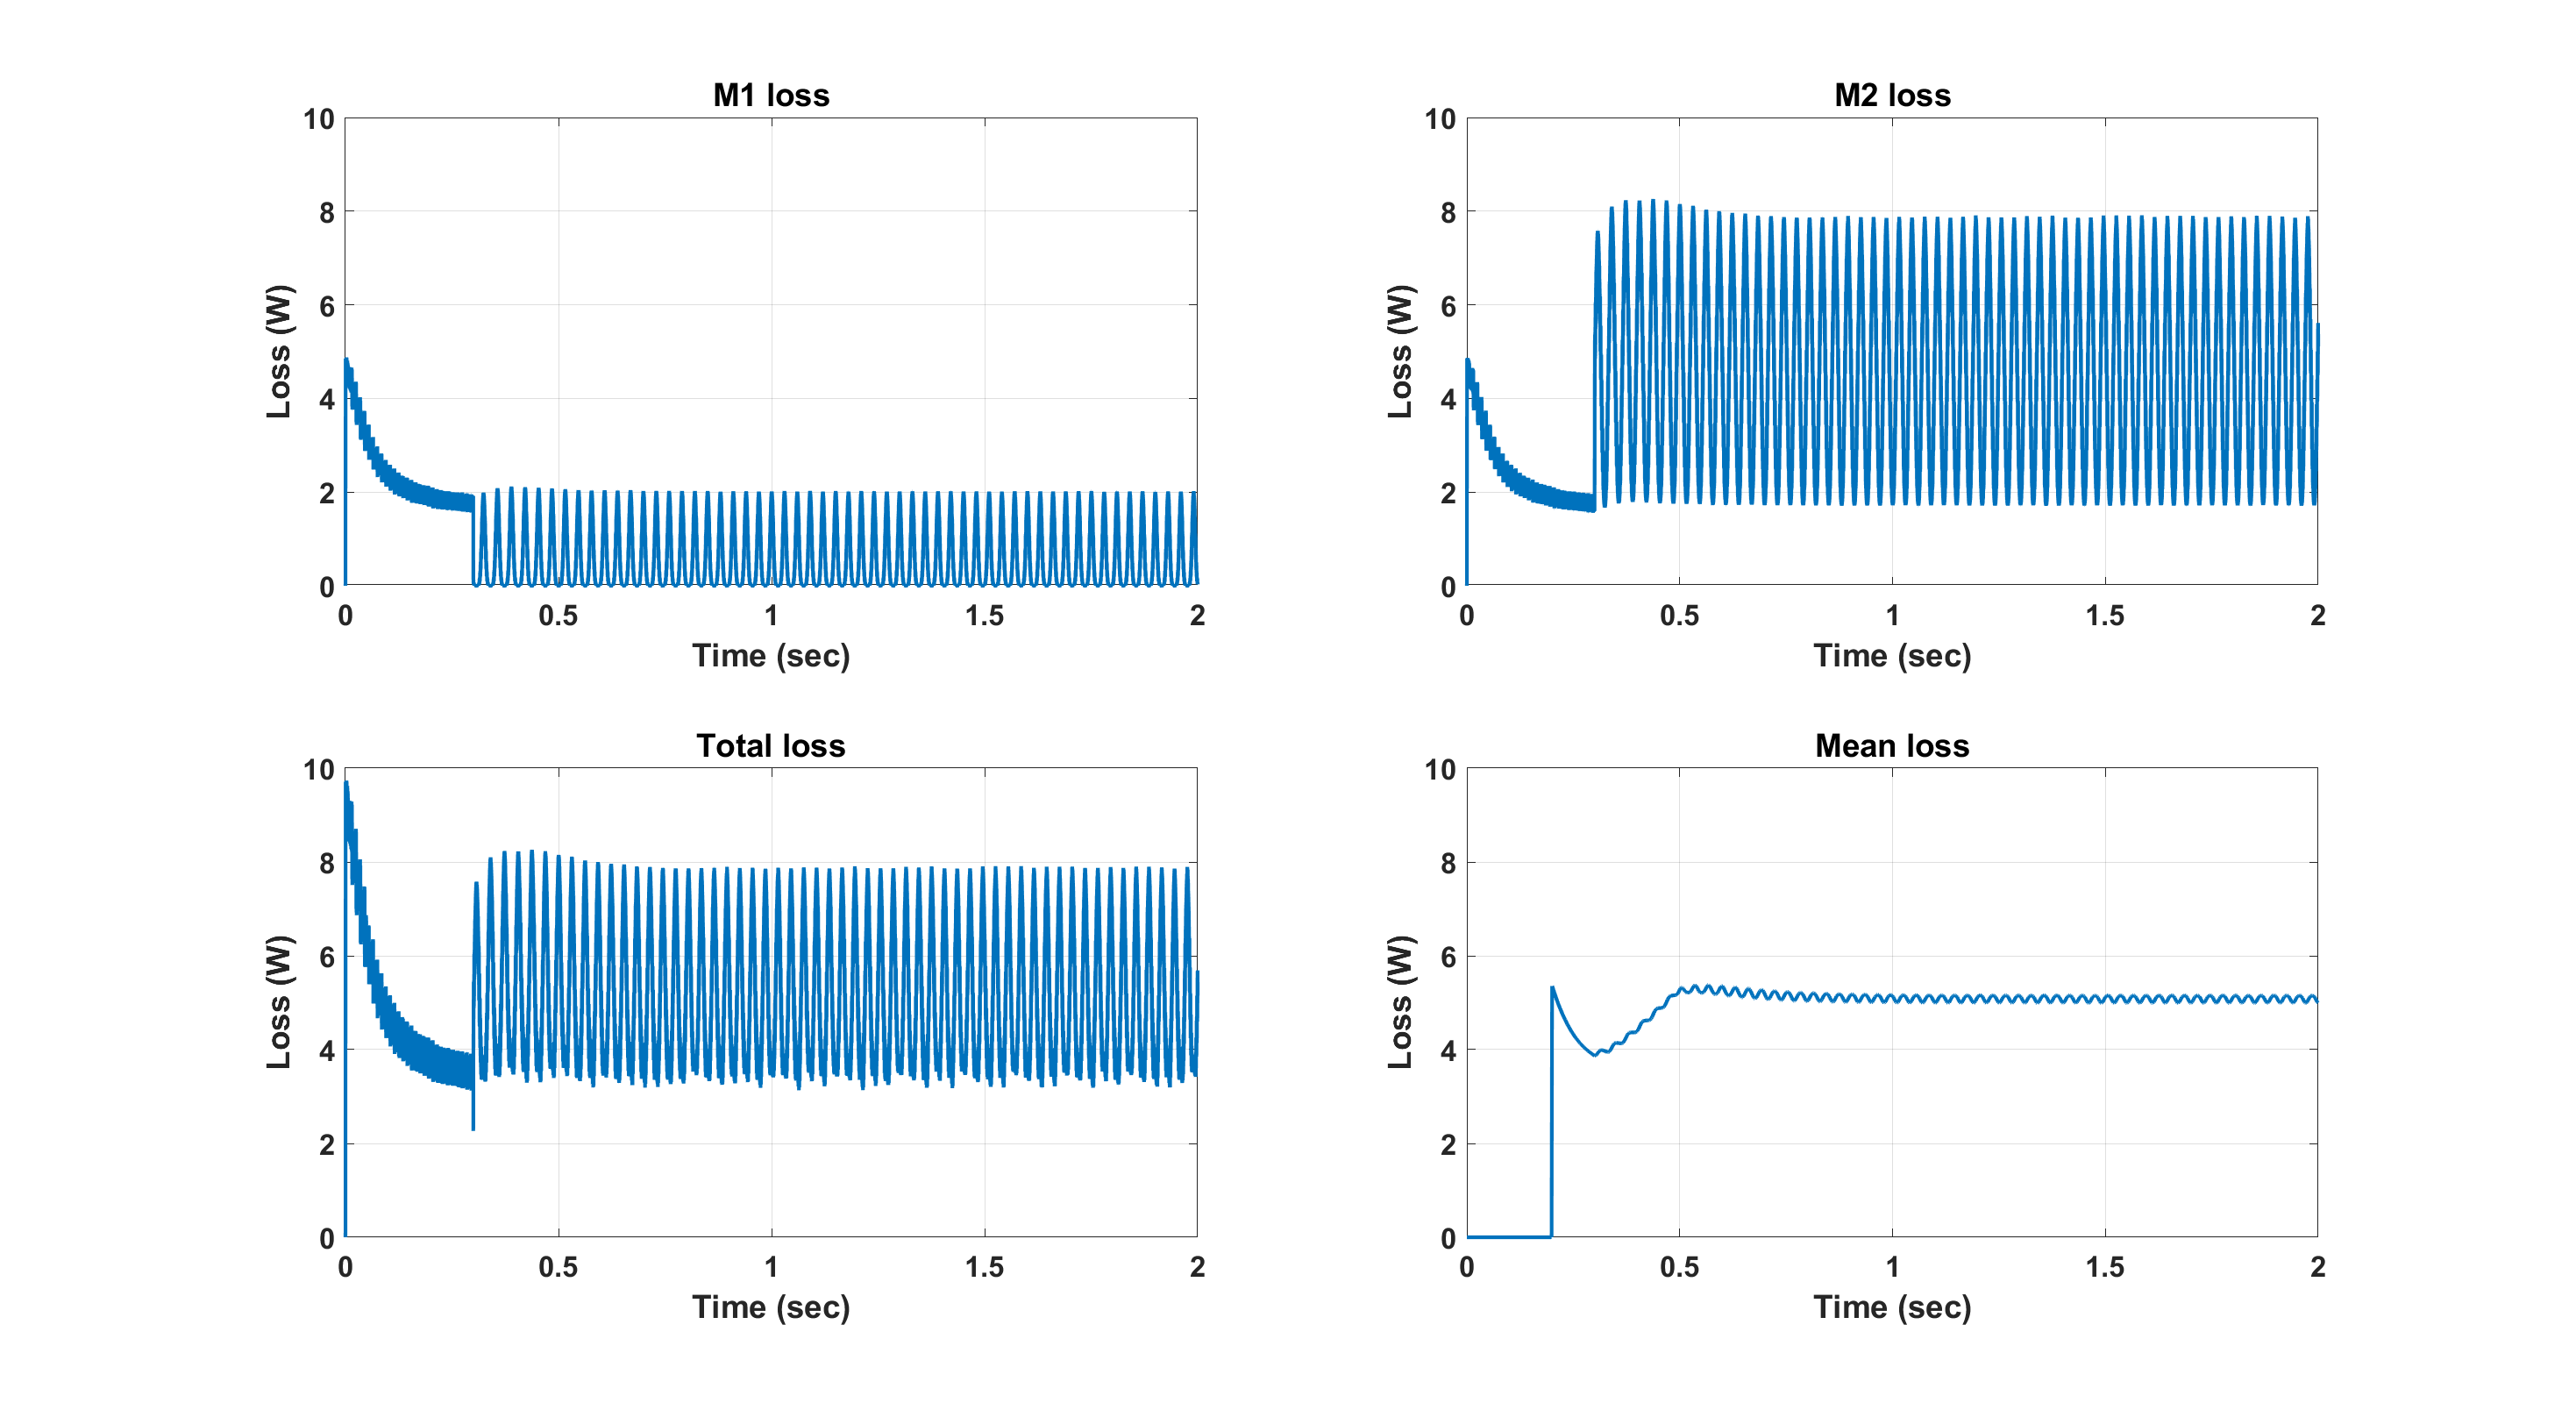
\includegraphics[scale=0.35]{SimulationResults/MyMethod/Loss.eps}
\caption{Module Losses for My Method}
\label{fig:LossMyMethod}
\end{figure}

\begin{figure}[H]
\centering
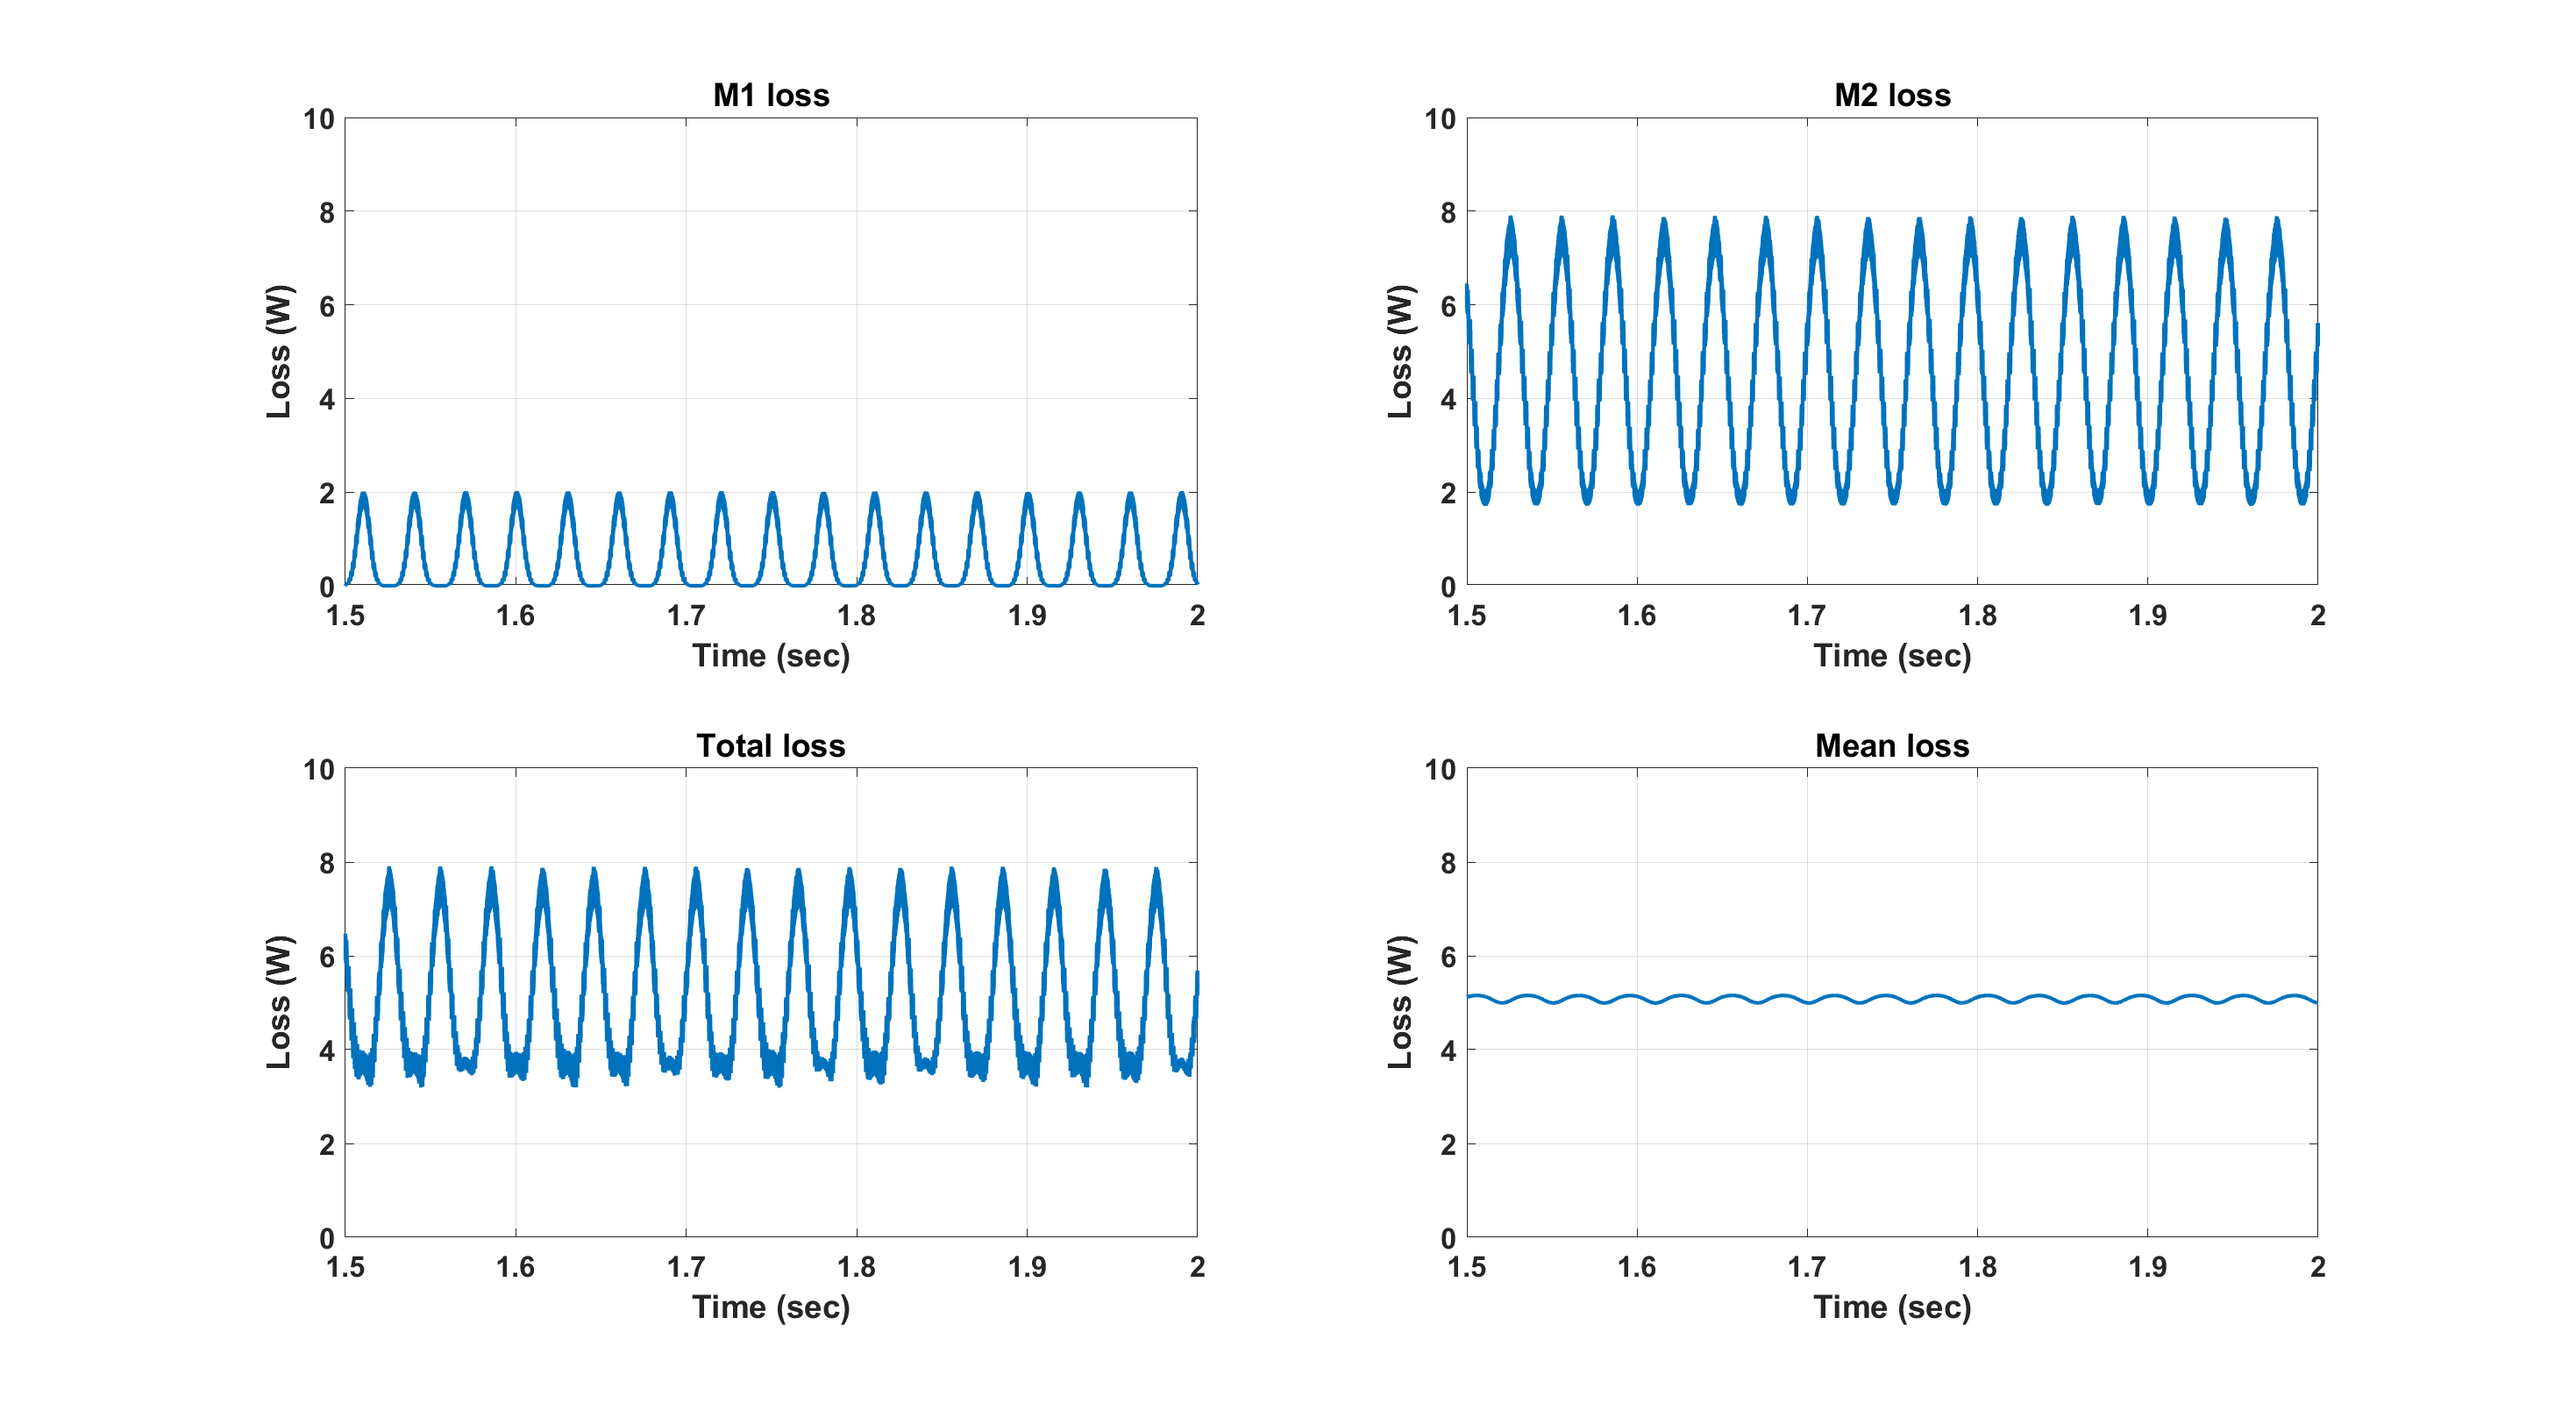
\includegraphics[scale=0.35]{SimulationResults/MyMethod/Loss_closer.eps}
\caption{Module Losses for My Method Closer}
\label{fig:LossMyMethodCloser}
\end{figure}

\begin{figure}[H]
\centering
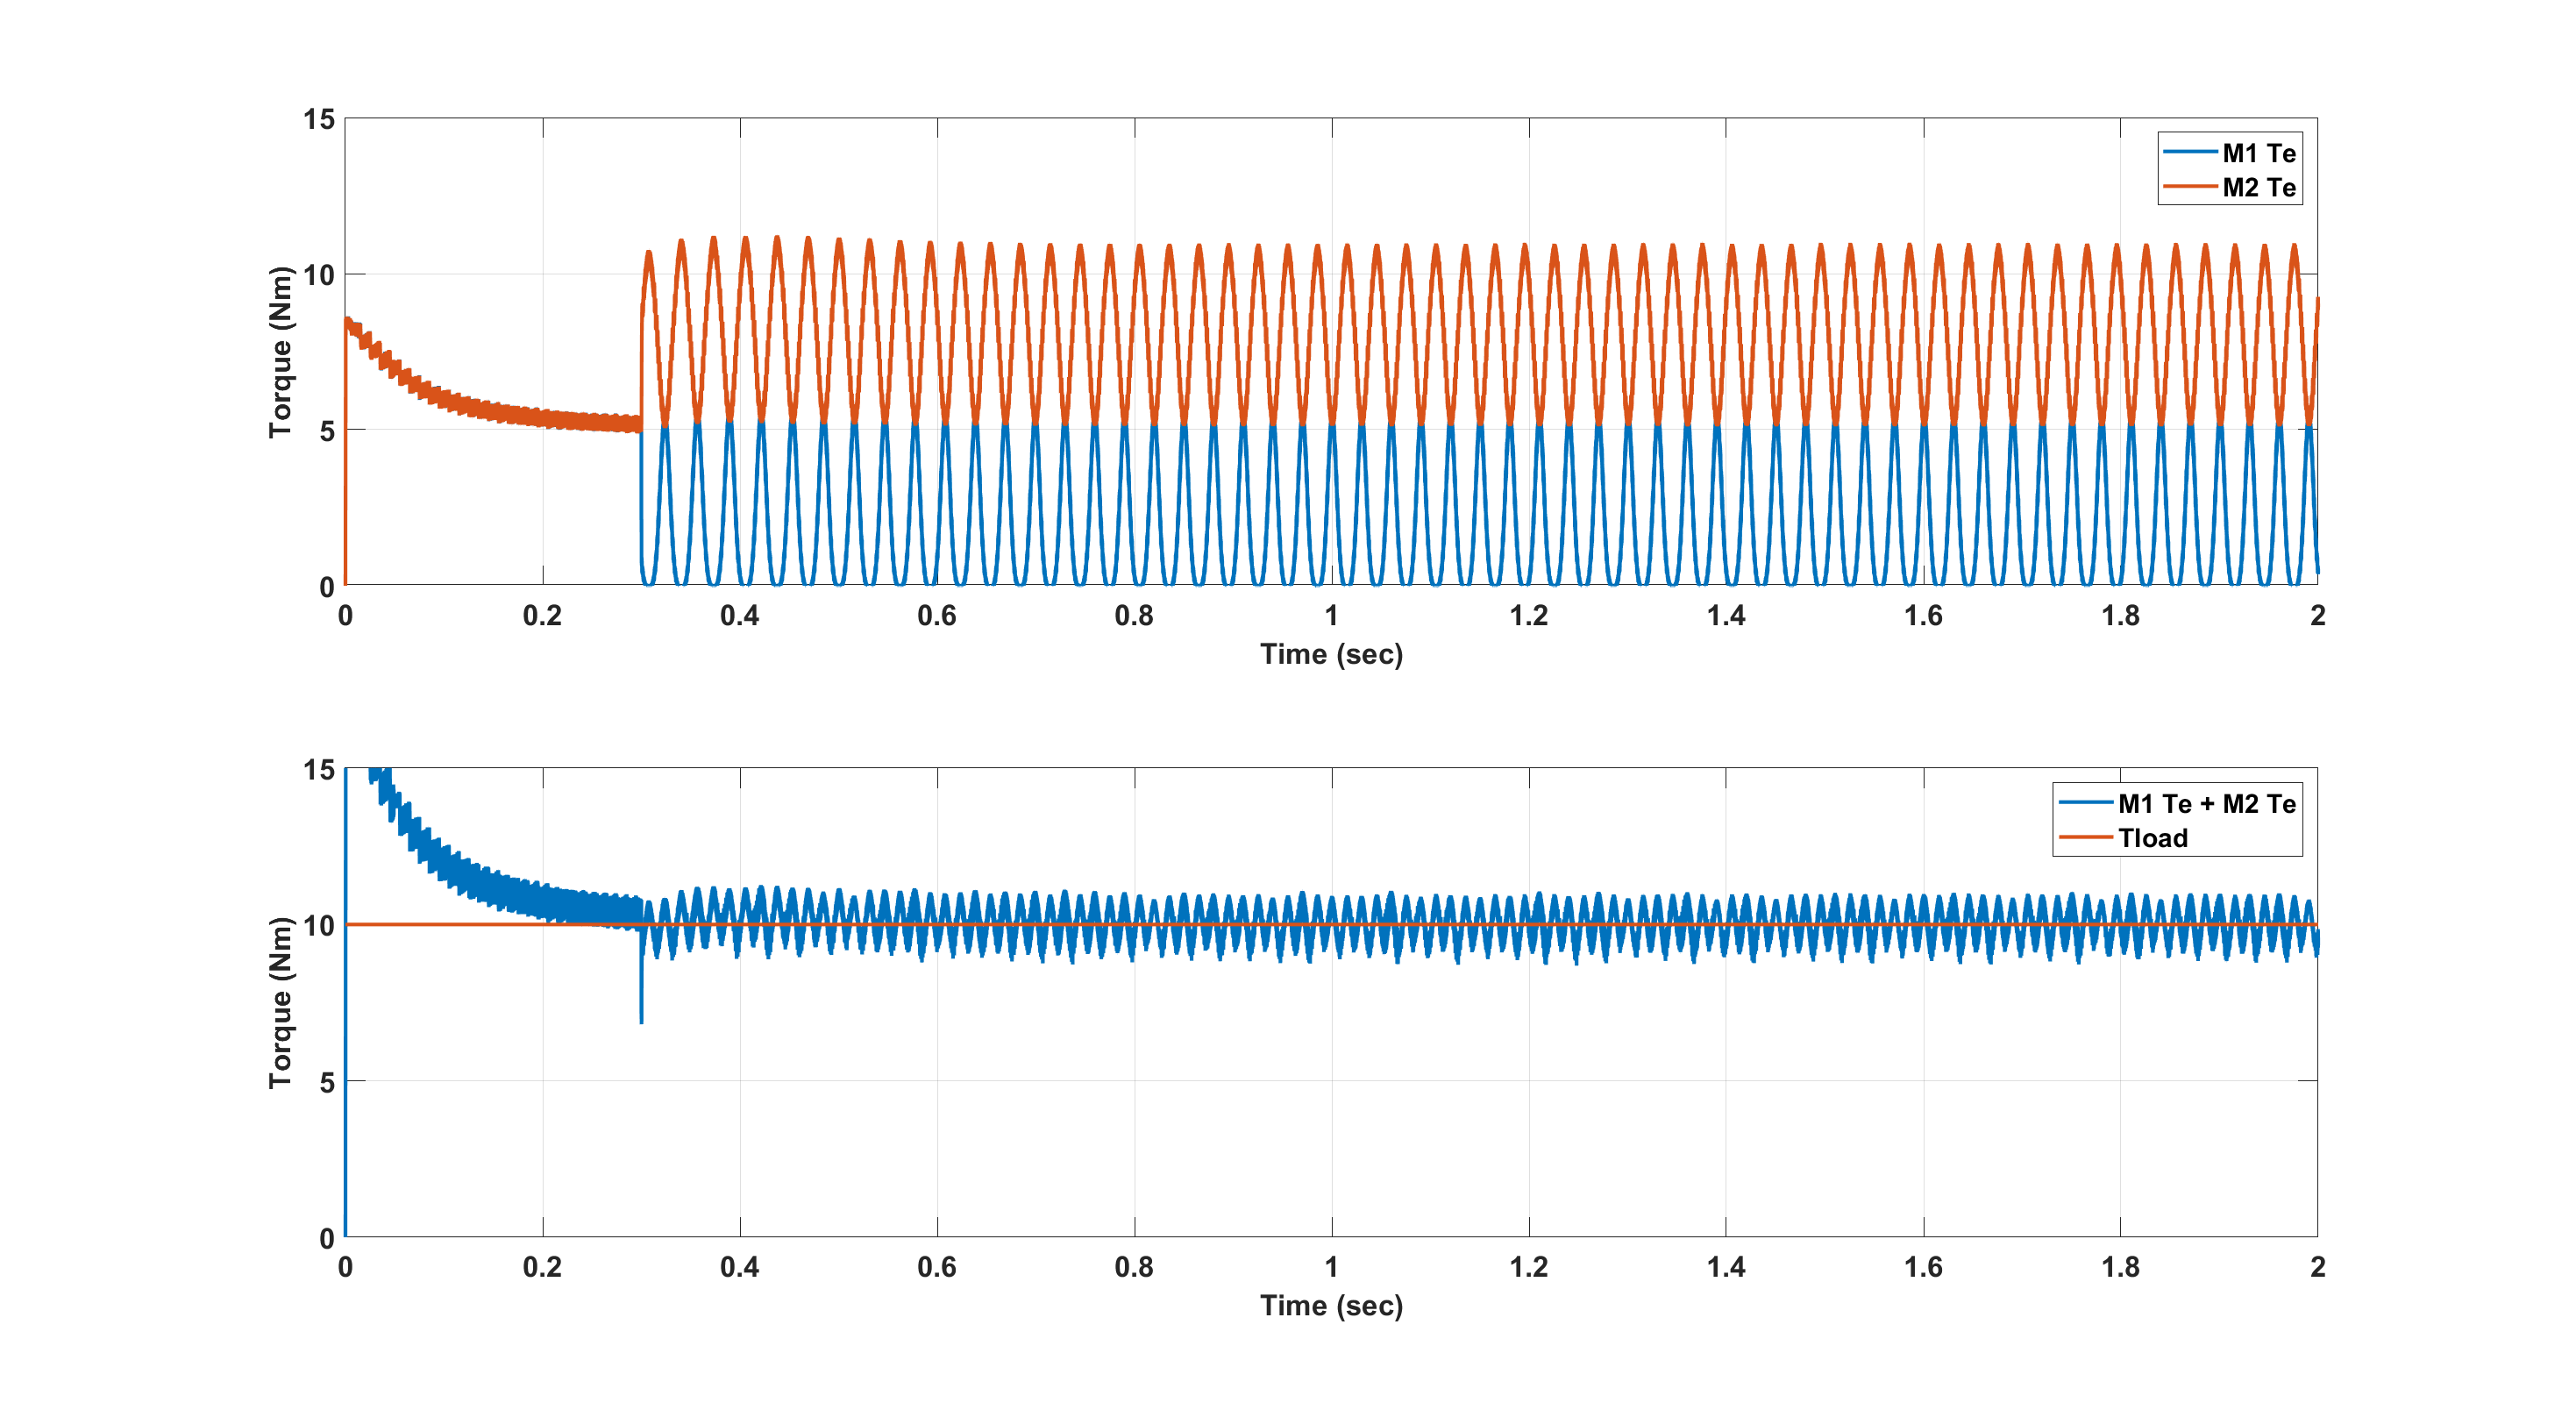
\includegraphics[scale=0.35]{SimulationResults/MyMethod/Torques.eps}
\caption{Module Losses for My Method}
\label{fig:LossMyMethod}
\end{figure}


\bibliographystyle{plain}
\bibliography{references}
\end{document}
